\documentclass[12pt]{iopart}
%\documentclass{article}

\usepackage{amsmath}
\usepackage{amscd}
\usepackage{amssymb} 
\usepackage{amsfonts}     
\usepackage{amsthm}
\usepackage{amsfonts} 
\usepackage{amsthm} 

\usepackage{tikz}
\usetikzlibrary{arrows,snakes,backgrounds}
% \usepackage{circuitikz}
% \usepackage{pgf}
% \usetikz
\usepackage{subfig}

\usepackage{algpseudocode}
\usepackage{algorithm}

\usepackage[super]{nth}
\usepackage{appendix}
% \usepackage{listings}
\usepackage{color}

\usepackage{hyperref}
%\usepackage{url}

\usepackage{cleveref}
\usepackage{cancel}
\usepackage{slashbox}

\usepackage{aviolov_style}
\usepackage{local_style}

\usepackage{iopams}

% \newtheorem{thm}{Theorem}[section]
% \newtheorem{lemma}{Theorem}[thm]
% \theoremstyle{definition}
% \newtheorem{ex}{Example}[thm]
% \newtheorem{defn}{Definition}[thm]

% \def\includegraphic{}
% \def\includegraphics{}
 
\begin{document} 

\title{Stochastic Optimal Control of Single Neuron Spike Trains}
\author{Alexandre Iolov$^{1,2}$, Susanne Ditlevsen$^2$, Andr\'e Longtin$^{1,3}$ 
		}	
\address{%
     (1) Department of Mathematics and Statistics, University of Ottawa, Ottawa,
    Canada
\\
    (2) Department of Mathematical Sciences, University of Copenhagen,
Copenhagen, Denmark
\\
    (3) Department of Physics, University of Ottawa,
    Ottawa, Canada
}
\ead{aiolo040@uottawa.ca}			
% \address{Department of Mathematics and Statistics, University of Ottawa, Ottawa, Canada 
% \\ Department of Mathematical Sciences, University of Copenhagen, Copenhagen,
% Denmark }
% \ead{$<$\href{mailto:aiolo040@uottawa.ca}
% 		{aiolo040 at uottawa dot ca}$>$}

% \date{\today}

\begin{abstract}

{\em Objective.} External control of exact spike times in single neurons is
important for basic understanding of neuronal activity, and has potential in
brain-machine interfaces, for improving neural prostheses, and in medical
applications related to neuronal disorders, such as Parkinson's disease or
epilepsy. The goal of this paper is the design of optimal controlled electrical
stimulation patterns to a cell to achieve a target spike train under
physiological constraints not to damage tissue. {\em Approach.} We pose a
stochastic optimal control problem to precisely specify the spike times in a
noisy leaky integrate-and-fire model of a neuron. In particular, we allow for
the noise to be of arbitrary intensity. The optimal control problem is solved
using Dynamic Programming if the controller has access to the voltage
(closed-loop control) and using a Maximum Principle for the transition density
if the controller only has access to the spike times (open-loop control). {\em
Main results.} We have developed a stochastic optimal control scheme to obtain
precise spike times, which is not limited by the intensity of the noise in the
system and is applicable in both the supra-threshold and sub-threshold regimes.
Given this scope, our simulations show that our algorithms produce the desired results. They further reveal that the numerical demands are non-trivial,
such that the algorithms may require efficiency refinements to achieve real-time
control, in particular the open-loop context is more numerically demanding than
the closed-loop one. Furthermore, we show how wrong the control strategy can
perform if we assume that the noise is negligible. {\em Significance.} More
precise targeting and control of neural activity to achieve optimal performance
in a noisy environment, in which most neurons are embedded, have great potential
in health care. The main contribution is the online feedback control of a noisy
system through modulation of the input, taking into account physiological
constraints on the control, as well as incurred costs to diminish adverse
effects.

\end{abstract}
% \tableofcontents MSC KEYS: 49N90 90C39 93E20 93C20 93C95

\maketitle

% \tableofcontents
% TODO: Remove ToCs (for internal consumption only)

\section{Introduction}
Manipulation of individual neurons through external electrical
stimulation provides a means to
controlling the spiking activity. Applications may arise, for
example, in brain-machine interfaces or in artificial prosthetics.
A natural goal is to make a cell produce a pre-specified spike train,
under certain constraints on the modulation of the input.
We consider this problem in the framework of Stochastic Optimal Control and
give both a feedback solution (closed-loop), when the cell voltage is
explicitly observable, as well as an open-loop solution when only the
occurrence of spikes is observable. Importantly, we allow for an
arbitrary noise intensity.

Both theoretically and in practice related problems have been
addressed in the literature. One objective has been to
obtain either minimum or maximum interspike intervals lengths,
when the input is constrained to be between some prespecified upper
and lower bounds, see e.g. \cite{Lee1994,Lefebvre1987} for a
mathematical treatment, or \cite{Danzl2009,Nabi2012,Wu2009} in a neuronal
context. Another objective is to break a pathological synchronous
firing pattern in clusters of neurons, highly relevant for neurological
disorders such as epilepsy and Parkinson's disease,
\cite{Nabi2013a,Nabi2011}, see also \cite{Feng2007b}.

Our objective, namely targeting exact spike times in single neurons, has been
considered mainly in the open-loop context, and in either absence of or for
small noise. In \cite{Ahmadian2011} they use the Spike Response Model,
\cite{Gerstner2002}, to control output target spike trains and implement their
scheme on pyramidal cells in mouse cortical slices. Their method is numerically
efficient and allows for the simultaneous control of many neurons. However the
efficiency of the numerics strongly relies on the assumption that the diffusion
noise, the value of $\b$ in \cref{eq:X_evolution_uo} below, is small enough, see
the discussion above and below equation 12 in \cite{Ahmadian2011}. They only
work with open-loop control. The difference between the objective in
\cite{Ahmadian2011} and what we consider below is that they maximize the
probability of spiking at some given time $t^*$, whereas we minimize the mean squared
difference between the realized spike time, $T_{sp}$ and the desired, $t^*$.
Moehlis et al. \cite{Moehlis2006} work with a Phase Response Model to obtain
spikes at exact times, while keeping the root mean square of the input to a
minimum. A similar approach is taken in \cite{Dasanayake2011}. They do not
consider noise, though, and only work with open-loop control. In
\cite{Nabi2013}, their methods are implemented on brain slices of pyramidal
neurons of rat hippocampus. While the
Phase Response Curve Model is a parsimonious and effective way to describe a
neuron's response to a stimulus, it is only valid in the supra-threshold regime,
where the unstimulated neuron is periodically spiking. Reference
\cite{Feng2003} investigates the control of the firing times of a
leaky integrate-and-fire neuron by varying the intensity of a noise process that
drives the voltage (there is no other intrinsic noise in the model). 
To obtain a given spike time, they choose the objective of minimizing the
variance of the membrane potential at the desired spike time, while forcing the
mean of the membrane potential at this time point to equal the threshold. This
provides exact solutions since it does not involve first-passage times, but has
the drawback that there is a non-negligible probability that the obtained spike
time will be far from the desired spike time.

Our objective of imposing a certain timing sequence for the spike train using an
externally applied control is obtained in both the closed- and
open-loop setting, and we specifically include the noise in the
calculations of the controls. We restrict the controlled input to stay
within pre-specified bounds, and also include a cost function to
minimize intervention.
Our main contributions are that we specifically allow for a non-negligible
noise component in the neural activity when calculating the control, and
consider both open- and closed-loop controls. In particular we do not
restrict our attention to the autonomously-spiking, supra-threshold regime. 

The paper is structured as follows: First we describe the neuron model and
formalize the control objective. Then we describe a feedback-based solution,
which assumes that the controller has detailed access to the voltage trajectory.
Then we relax the observation assumption so that the controller only has access
to the spike times. Finally, we compare the two methods through
simulations against a simple-minded control technique which ignores
the stochastic input to the neuron.

\section{Problem Formulation}
A basic but useful model for the neural membrane potential evolution is the
noisy leaky-integrate-and-fire model:
\begin{equation}
\begin{gathered}
dX(t) = \left(\Iext(t) - \frac{X(t)}{\tc} \right) \intd{t} + \b \intd{W},
\\
X(0) = 0,
\\
X(\ts) = \xth \implies
\begin{cases}
X(\ts^+) = 0. & 
\end{cases}
\end{gathered}
\label{eq:X_evolution_uo}
\end{equation}
Here $X(t)$ represents the membrane electric potential at time $t$, which in
absence of input decays to $0$ with a time constant of $\tc$, $dW$ is a Brownian
motion increment scaled by $\b$ and $\Iext(t)$ is the deterministic external input to the cell. Having last
spiked at time $0$, the potential hits $\xth$ at some random time $\ts$, the
potential resets to $0$ and the process starts all over again. 
We write $\ts^+$ for the limit from the right at $\ts$.
Throughout the paper the threshold is set to one, $\xth = 1$.

Suppose that we have some control over the external current such that it can be
decomposed as
\begin{equation}
\Iext(t) = \m + \a(t),
\label{eq:current_mu_alpha}
\end{equation}
where $\m$ is an uncontrollable, but constant part of the external current and
$\a(t)$ is controllable, i.e.\ it can be chosen to achieve some goal.
A natural goal is to attempt to control the spike time, $\ts$.
That is, how do we choose $\a(t)$ such that $\ts \approx \T$, where $\T$ is the
desired spike-time. A natural optimal control objective to achieve this is the
least squares solution
\begin{equation}
\a(\cdot) = \argmin_{\a(\cdot)} \{\, \Exp[(\ts- \T)^2] \,\},
\label{eq:OC_LS_variance}
\end{equation}
where expectation is taken with respect to the distribution of the trajectories
of $X$.

Often the control has certain constraints. The most common are simple box
constraints:
\begin{equation}
\a(t) \in [\amin, \amax] \quad \forall t.
\label{eq:bound_constraints_alpha}
\end{equation}

% \subsection{Optimal Control Formulation}
In addition to \cref{eq:OC_LS_variance}, we will also add to our objective a
running energy cost based on the control. This regularizes the problem
eliminating the subtleties of singular-control situations and it serves to avoid excessive
control as well as to avoid excessive charge building up on the cell, see
\cite{Ahmadian2011}. 

So we seek an optimal control, $\a^*$, that solves
\begin{align}
J[\a(\cdot)] =&
\Exp\left[
\e \int_0^\ts  \a^2(s) \intd{s}
+
(\ts - \T \big)^2 \right]
\label{eq:OC_LS_variance_energy}
\\ \notag
\a^*(\cdot) =& \argmin_{\a(\cdot)} J[\a(\cdot)],
\end{align}
where $\e$ measures how much weight we put on minimizing the energy cost.
If $\e = 0$, then we do not care at all about the expended energy cost.

It will often be the case that $\a$ means either a function or a
value of that function at a particular time. This function could be
random, i.e.\ a stochastic process. Since $\a$ is used to control the behaviour
of $X$, it will be at least measurable with respect to the filtration of $X$,
see Ch.\ 11 in \cite{Oksendal2007} for the details. We will try to make clear
below when we are refering to $\a$ as a stochastic process and when we are merely refering to its particular
value at some time. For example, in \cref{eq:OC_LS_variance_energy}, $\a(\cdot)$
refers to the function, while $\a(s)$ refers to that function's value, possibly
random, at time $s$.

We will consider two control contexts -- {\sl closed-loop} and  {\sl open-loop}
control. In closed-loop control, the value of $X$ at time $t$ is observable
and can be used in determining the control. In open-loop control only the spike
times are observable. In the closed-loop context, we write the control as $$\a =
\a(x,t)$$ to indicate its dependence on $X(t)$ and to express that it will be
updated based on the time-course of $X$. In the open-loop context, we write $$\a
= \a(t)$$ to indicate that $\a(\cdot)$ is decided for all times at time 0. The
techniques used to obtain the optimal controls in the two scenarios will be
different. For the closed-loop scenario we use Dynamic Programing,
see \cite{Fleming1975}, while for the open-loop scenario we use a form of the
Maximum Principle applied to the transition density of the controlled process,
see \cite{Borzi2012}.

Crucially, we assume that the model parameters, $\m,\tc,\b$ in
\cref{eq:X_evolution_uo,eq:current_mu_alpha} are known. This is a strong assumption and will be
discussed later. 

\subsection{Parameter Regimes}
Different  parameter regimes can be envisioned given \cref{eq:X_evolution_uo},
depending on whether the noise intensity, $\b$, is
relatively high or low, and whether the external, uncontrollable bias current,
$\m$, induces spikes in the absence of noise or not. 
Spikes will occur in the absence of noise, if and only
if $ \m > 1 / \tc,$ which is called the supra-threshold regime. When $\m
\leq 1/\tc$, the regime is called the sub-threshold regime.
In addition we will investigate two values of $\b$, which we
will call high-noise and low-noise, respectively.
Example values for each parameter regime are given in \cref{tab:regimes}, and we
visualize a single path for each regime in \cref{fig:regime_path_examples}.
\begin{table}
\begin{tabular}{|l||{c}|{c}|}
\hline
\backslashbox{$\m$}{$\b$}
& $1.5$ & $0.3$ \\
\hline
$1.5 / \tc $ &Supra-threshold-High-noise & Supra-threshold-Low-noise \\
\hline
$0.1 / \tc$   &Sub-threshold-High-noise & Sub-threshold-Low-noise \\
\hline
\end{tabular}
\caption{Regime labels and example values. Note that for the numerical
experiments below, we use $\tc = 0.5$}
\label{tab:regimes}
\end{table}
%\usepackage{graphics} is needed for \includegraphics
\begin{figure}[htp]
\begin{center}
  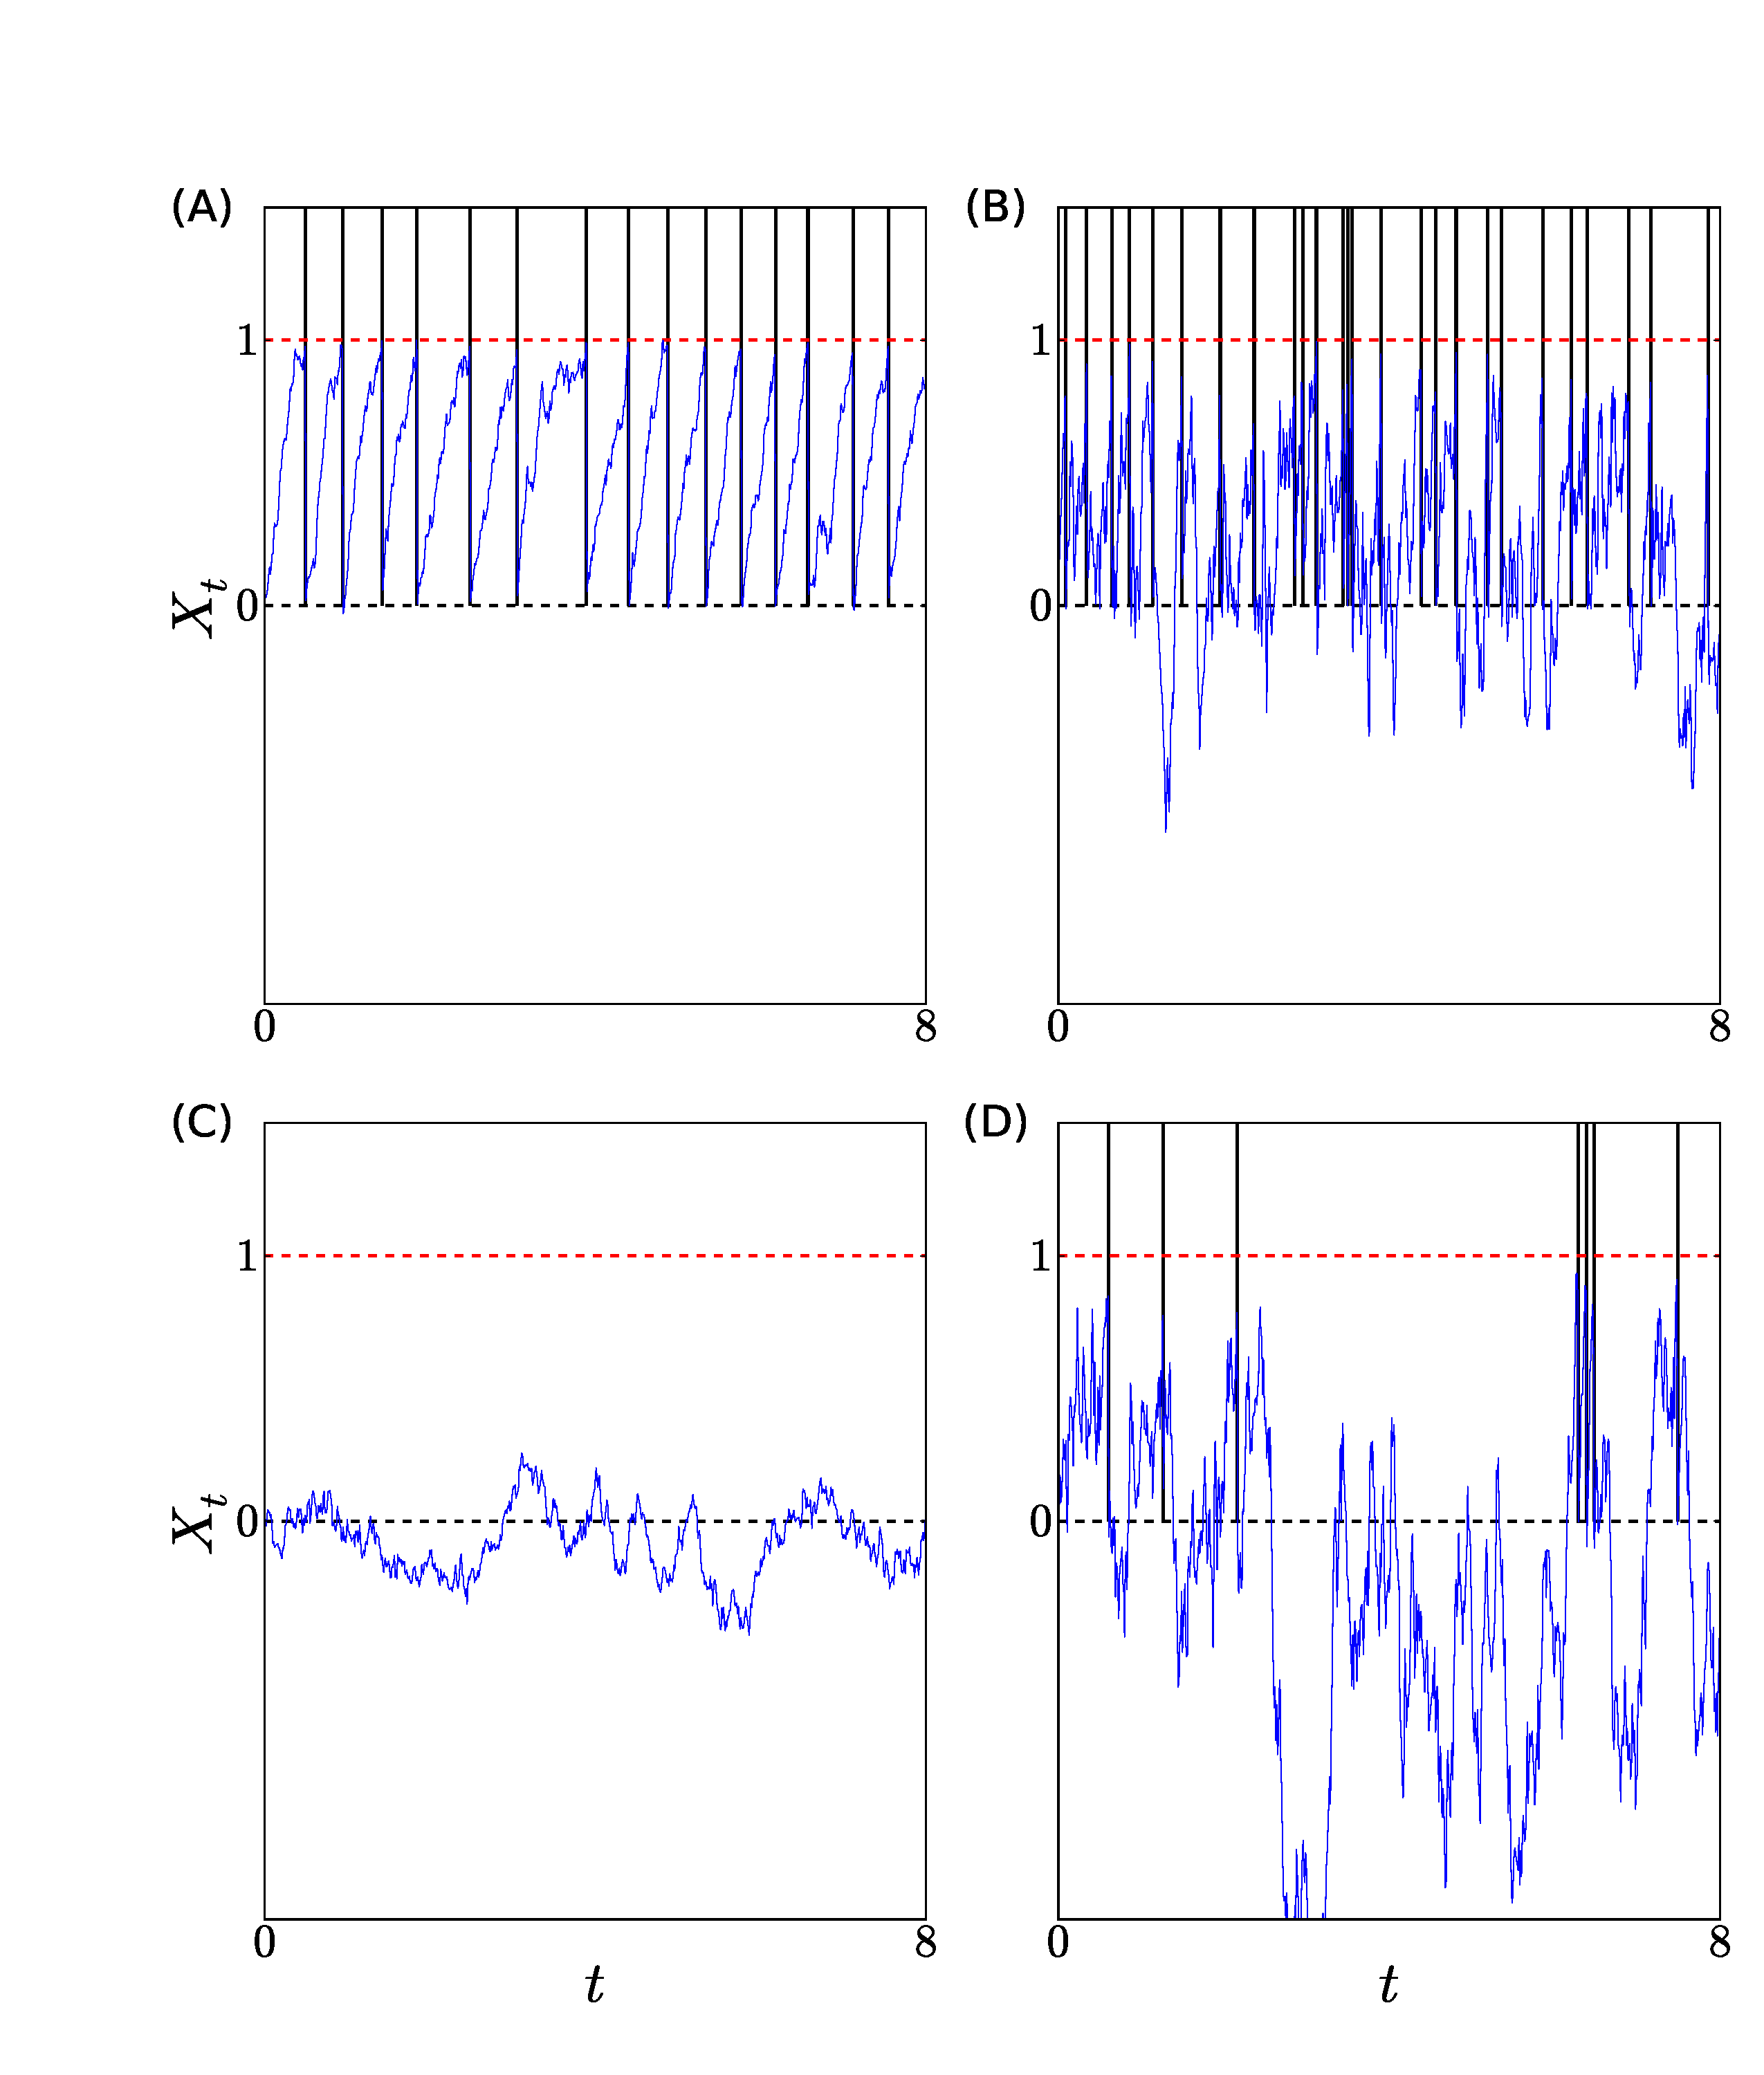
\includegraphics[width=0.99\textwidth]{Figs/PathSimulator/path_T=14_combined.pdf}
  \caption[labelInTOC]{Example Trajectories from \cref{eq:X_evolution_uo}
  using the parameter values from \cref{tab:regimes}. 
  A) Supra-Threshold-Low-Noise 
  B) Supra-Threshold-High-Noise 
  C) Sub-Threshold-Low-Noise
  D) Sub-Threshold-High-Noise. 
  Note the multiple crossings very close together in the high-noise regimes
  in B and D. }
  \label{fig:regime_path_examples}
\end{center}
\end{figure}

\section{Closed-Loop Solution - Dynamic Programing}
We now detail the Dynamic Programing approach to obtaining an optimal feedback
control. In closed-loop, the controller can be continuously updated depending on
the realization of the stochastic process, $X$.

Given a time $t$ and a realized voltage value $X(t) = x$, let $(\ts-t)$ be the
unknown and random remaining time to spike, note that $\ts$ is a random
variable. Given arbitrary $t, x$, our remaining-cost objective, $J[\a(\cdot);
x,t]$, will be
\begin{equation}
J[\a(\cdot); x,t]  =
\Exp\left[
\big((\ts-t) - (\T-t) \big)^2  
+
\e \int_t^\ts  \a^2(s) \intd{s} 
\,\Big|\, X(t) = x
\right],
\label{eq:OC_LS_cost_to_go}
\end{equation}
i.e.\ if time $t$ has elapsed without a spike, we now want to minimize
the difference between $(\ts - t)$ and $(\T-t)$, given the current state $x$.
The mean in \cref{eq:OC_LS_cost_to_go} is taken over the distribution of
hitting times, $\ts$, conditional on $X(t)$ or equivalently over the
distribution of forward trajectories of $X$ starting at $x$ and ending at the
threshold. 
Recall that in the closed-loop scenario, we assume that
the value of $X(t)$ is known to the controller. A similar problem is discussed
analytically at length in the book on optimal control by Peter Whittle,
\cite{Whittle1996}, although there is no discussion there of the numerics
required to solve it. 

\subsection{Hamilton-Jacobi-Bellman equation}
The Hamilton-Jacobi-Bellman (HJB) equation, see \cite{Fleming1975,Whittle1996}
or the articles \cite{Danzl2009,Nabi2013a} in a neuroscience context, associated
with the optimal control for \cref{eq:OC_LS_cost_to_go} is obtained as follows.
We introduce the value function, $\v(x,t)$, as the minimum of the remaining-cost objective, i.e.\ of
the cost function between the current time $t$ and the desired spike time
$\T$:
\begin{align}
\v(x,t) =&
 \min_{\a(\cdot)_{s \geq t}}
 \{J[\a(\cdot); x,t] \}
\notag
\\
=&
\min_{\a(\cdot)_{s \geq t}}
\Exp\left[
\big((\ts-t) - (\T-t) \big)^2
+
\e \int_t^\ts  \a^2(s) \intd{s}
\,\Big|\,X(t) = x
\right].
\label{eq:OC_LS_mean_value}
\end{align}
Then $\v$ satisfies the following HJB partial differential equation (PDE):
\begin{equation}
\begin{gathered}
\di_t \v(x,t) + \tfrac{\b^2}{2} \di_x^2 \v(x,t) + \\
\min_{\a(x,t) \in [\amin,
\amax]}\Big\{ \e \a^2 (x,t)+ \left(\m + \a(x,t)-\tfrac{x}{\tc}\right) \di_x
\v(x,t) \Big\} = 0.
\label{eq:OC_LS_mean_HJB}
\end{gathered}
\end{equation}
The special feature of \cref{eq:OC_LS_mean_HJB} in contrast to a generic
parabolic PDE is that it contains an embedded optimisation that depends on the
solution, $\v$. For each $x,t$ in the computational domain,
$\a$ is chosen such as to minimize $\{\e \a^2 + \left(\m + \a -
\tfrac{x}{\tc}\right) \di_x \v \}$. Here we can solve for the optimal control, $\a^*(x,t)$ analytically as:
\begin{align}
\a^*(x,t)  =& \argmin_{\a \in [\amin, \amax]}\big\{\e \a^2 + (\m + \a-\tfrac{x}{\tc}) \di_x\v\big\}
\notag
\\
=&
\min \left(\amax, \max\left(\amin, -\frac{\di_x\v(x,t)}{2\e}\right)\right).
\label{eq:OC_LS_variance_energy_quadratic_control}
\end{align}
With this the HJB PDE becomes
\begin{equation}
\di_t \v(x,t) + \tfrac{\b^2}{2} \di_x^2\v+
\e (\astar(x,t))^2 + (\m + \astar(x,t)-\tfrac{x}{\tc}) \di_x\v
= 0.
\label{eq:OC_LS_mean_HJB_bounded_control}
\end{equation}

We need to consider boundary conditions (BCs) for $\v$. If $X(t) = \xth$ then we
have a spike now and $\ts = t$. Thus $$ \v(\xth,t) = (t-\T)^2.$$ At the
threshold, the value function equals the squared difference between the desired
spike time and the realized one. For $x \ll 0$, we assume that $\v$ is not
significantly affected by the change in $x$, i.e.\ that $$ \di_x \v(\xmin, t) =
0 $$ for some lower boundary $\xmin$. Such a boundary condition will be
justified if we impose artificial reflecting boundaries for the diffusion at
$\xmin$. So we need to determine for which $\xmin$ is a reflecting boundary
consistent with the dynamics. For example, we can take $\xmin$ to be two
standard deviations below the mean of the stationary distribution of the
maximally inhibited, $\a=\amin$, \cref{eq:current_mu_alpha}. That is we set
$\xmin = \tc(\mu + \amin) - 2 \b / \sqrt{\tc/2}$. We further enforce
that $\xmin \leq -0.5$.
% Ooops, we need $\di_x\v\neq 0$ and here we are setting $\di_x\v= 0$ in one of
% the BCs\ldots oh well.

Note that Dynamic Programing and the HJB equation work backwards. Thus the
evolution of the value function proceeds from the future to the past and we need
some Terminal Condition (TCs) at some point in the future, possibly infinity,
from which to start incrementing $\v$ using the dynamics and the BCs. To
determine TCs for $\v$, our idea is simple: if we reach $\T$ without having
spiked we apply maximum control in the positive direction, i.e.\ 
$$t>\T \implies \a(t) = \amax.$$ Thus: \begin{equation}\v(x,\T) = \Exp
\Big[\trem^2 \,\Big|\, X(\T) = x, \a(t) = \amax \Big].
\label{eq:valuefun_TCs}
\end{equation}
Note that we are making an approximation here
- we are ignoring the energy term, $\eps u^2$, in the objective for
$t>\T$. Naturally, this approximation is ever more accurate for $\eps \ll 1$.
We discuss in more detail the validity of the approximation in
\cref{sec:effect_of_eps}.
Alternatively, we could impose this approximate terminal condition at some $t^+
> \T$.

We will see the quantity on the right hand side of \cref{eq:valuefun_TCs}
repeatedly so we will give it a special name.
\begin{equation}
\Ttwo(x) := \Exp \Big[\trem^2 \,\Big|\, X(\T) = x, \a(t) = \amax \Big].
\label{eq:Trem_squared}
\end{equation}
$\Ttwo$ is the second moment of the remaining time to reach the
threshold starting at $X(\T) = x$ and applying $\amax$ throughout. This quantity
can be found easily for all $x$ in the domain by solving a stationary backward Kolmogorov
equation. This is an extension to the calculation of the first moment of an
exit-time as seen in textbooks such as \cite{Jacobs} and we give the
details in \ref{sec:valuefun_TCs}.

Thus, we restate the HJB equation in its fully specified form:
\begin{equation}
\begin{gathered}
\di_t \v(x,t) + \tfrac{\b^2}{2} \di_x^2\v(x,t)+
\e \a^2(x,t) + \big(\m + \a(x,t) -\tfrac{x}{\tc}\big)\cdot \di_x\v(x,t)
= 0,
\\
\a (x,t) = \min \left(\amax, \max\left(\amin, -\frac{\di_x \v(x,t)}{2\e}\right)
\right).
\\
\begin{cases}
\v(\xth,t) = (t-\T)^2  \quad & \textrm{upper BC}
\\
\di_x \v(\xmin, t)  = 0  \quad &\textrm{lower BC}
\\
\v(x,\T)  =
% \Exp \Big[\trem^2 \,\Big|\, X_\T = x, \a(t) = \amax \Big]
% \Exp[\t^2|x, \amax]  \quad
\Ttwo(x)
\,& \textrm{TC}
\end{cases}
\end{gathered}
\label{eq:OC_LS_HJB_full}
\end{equation}
We are solving $\v(x,t)$ over the domain $[\xmin, \xth] \times [0,\T]$.

\subsection{The numerical method for the HJB equation}
\label{sec:hjb_numerix}
We now have a PDE for $\v$ and an algorithm for computing all the BCs and TCs of
this PDE. It is time to discuss the numerical method for solving
\cref{eq:OC_LS_HJB_full}. Since it is one-dimensional in space, it is straight
forward to apply the standard centred finite difference using the
Crank-Nicholson scheme to step in time, see ch.\ 19.2 in \cite{Press1992}. To
resolve the non-linearity, $(\di_x\v)^2$, in the PDE, we treat it as a mixed
implicit-explicit term $$(\di_x \v(x,t_k))^2 = \di_x \v(x,t_k) \cdot \di_x
\v(x,t_k) \approx \underbrace{\di_x \v(x,t_k)}_{\textrm{implicit}} \cdot
\underbrace{\di_x\v(x,t_{k+1})}_{\textrm{explicit}}.$$ Note that the implicit
term is in the previous time $t_k$ instead of, as is conventional, the next
$t_{k+1}$, because we are solving for $\v$ {\sl backwards} in time from
$t_{k+1}$ to $t_k$ down to  $t_0 = 0$.

The numerical scheme is implemented in Python, using the Scipy/Numpy library,
\cite{Scipy}. For the discretization in time and space, we choose $\Delta x$ and
$\Delta t$ in relation to the parameter regimes. In particular, we take $\Delta
x$ to be less than $\b$ divided by the largest possible absolute value of $(\m +
\a - x/\tc)$ for $\a \in [\amin, \amax], x \in [\xmin, \xth]$; in our examples
this always be equal to $\mu + \amax - \xmin/\tc$. This is an attempt to ensure
that numerically we are in the diffusion-dominated regime. We set $\Delta t$ to
be twice the value of $\Delta x$ divided by the largest possible absolute
value of $(\m + \a - x/\tc)$. For example in the Supra-Threshold Low-Noise regime, we
have $\Delta x = 0.0043$ and $\Delta t = 0.0013$. In all regimes, our
discretization results in point-wise convergence of up to at least three
significant digits for the value function. We consider this to be a sufficiently
fine discretization.

We next demonstrate solutions for the value function and the associated
control law for a parameter set from each regime in \cref{tab:regimes}.

\subsection{Solutions of the HJB equation} 
We set $\T=1.5$ and $\eps = 0.001$, so that the primary focus is the accurate
spiking and energy minimization considerations are secondary.

In \cref{fig:HJB_4regimes_value_control_cuts}, we depict three snapshots in time
of the value function and the control, $\v$ and $\a$, at $t = [0,\T/2, \T]$,
i.e.\ at the beginning, middle and end of the relevant time interval. Then in
\cref{fig:HJB_4regimes_value_surf} we show the entire value function, $\v(x,t)$,
the solution to \cref{eq:OC_LS_HJB_full}, for each of the parameter regimes.
% THE CUTS:
\begin{figure}[htp]
\begin{center}
  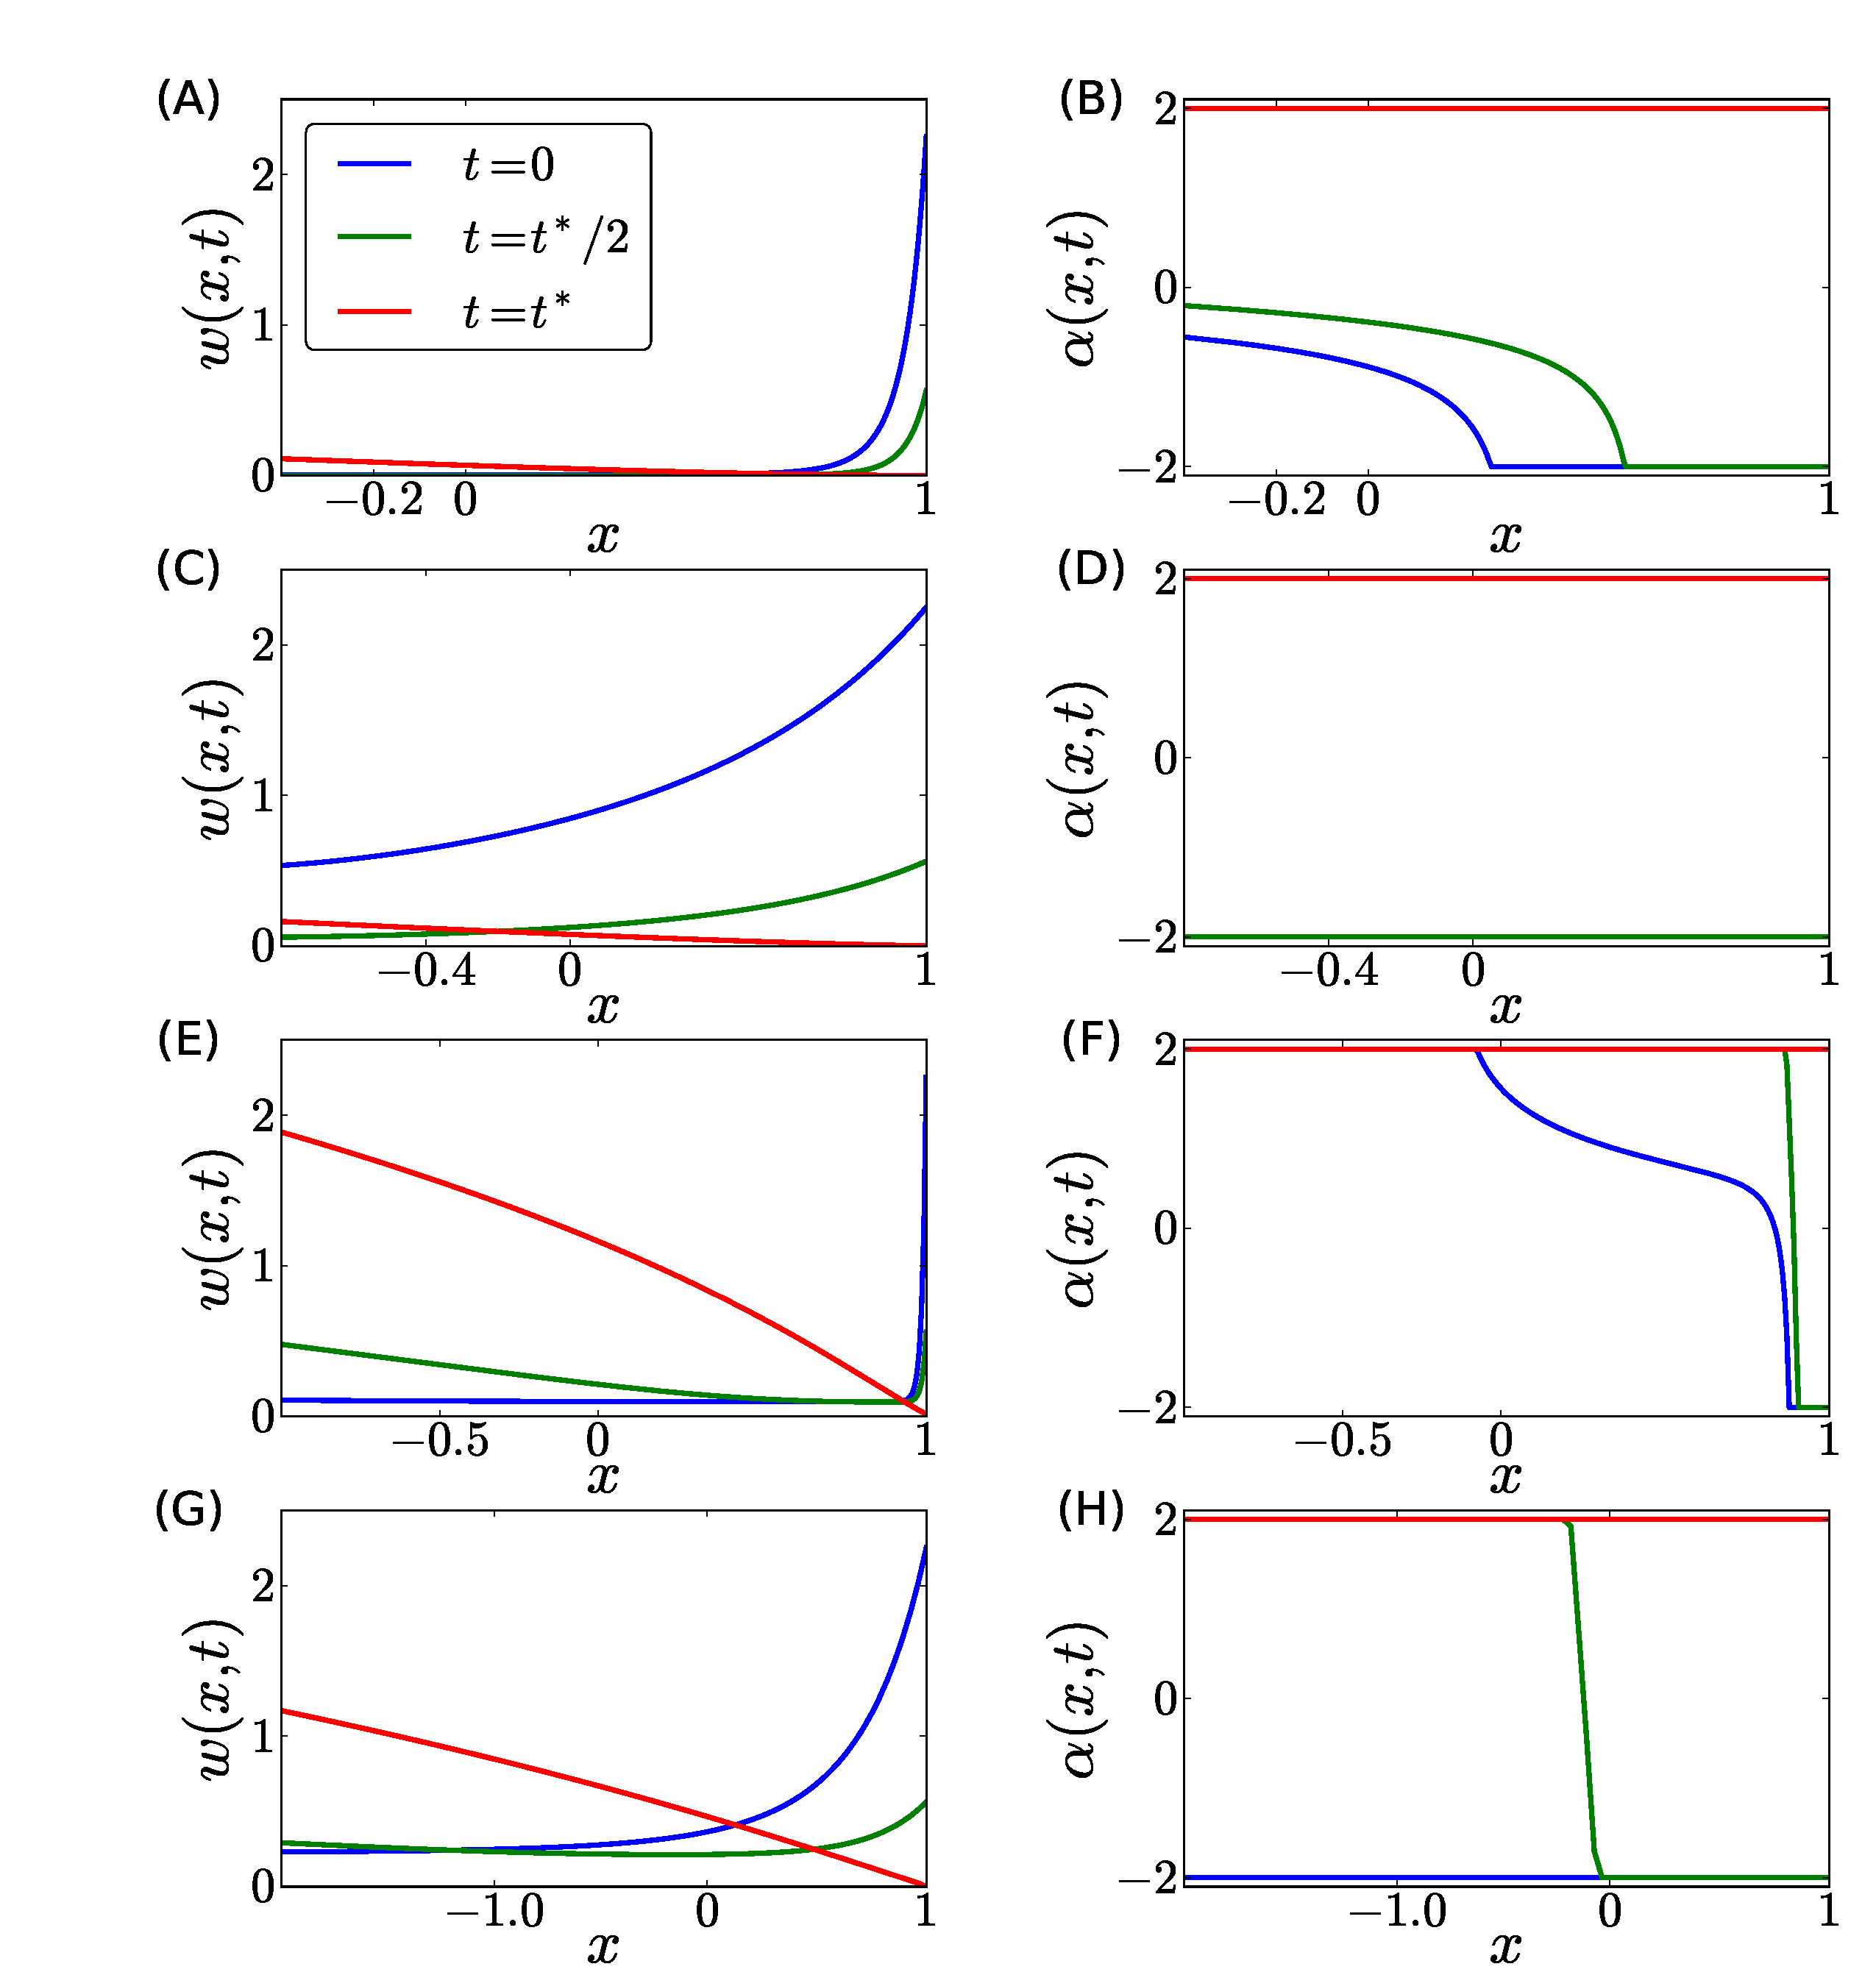
\includegraphics[width=\textwidth]{Figs/HJB/Regimes_vc_cuts.pdf}
  \caption[labelInTOC]{Snapshots of the value function, $\v$, on the left and on
  the optimal control, $\a$, on the right for $t$ fixed, at the start (blue),
  mid-point (green) and end-point (red), for each of the four regimes.
  The desired spike time is set to $\T=1.5$ assuming the previous spike was at
  $t=0$, the energy penalty, $\eps = 0.001$. The control bounds are $\a \in
  [-2,2]$. 
  Note that all red value function curves go to zero at the threshold to satisfy
  the upper BC in \cref{eq:OC_LS_HJB_full}.
  Note that the green and blue
  curves in F) are lying on top of each other for all $x$.
  \\
  A,B) Supra-Threshold-Low-Noise
  C,D) Supra-Threshold-High-Noise
  E,F) Sub-Threshold-Low-Noise
  G,H) Sub-Threshold-High-Noise
  }
\label{fig:HJB_4regimes_value_control_cuts}
\end{center}
\end{figure}
% THE SURFS:
\begin{figure}[h!]
\begin{center}
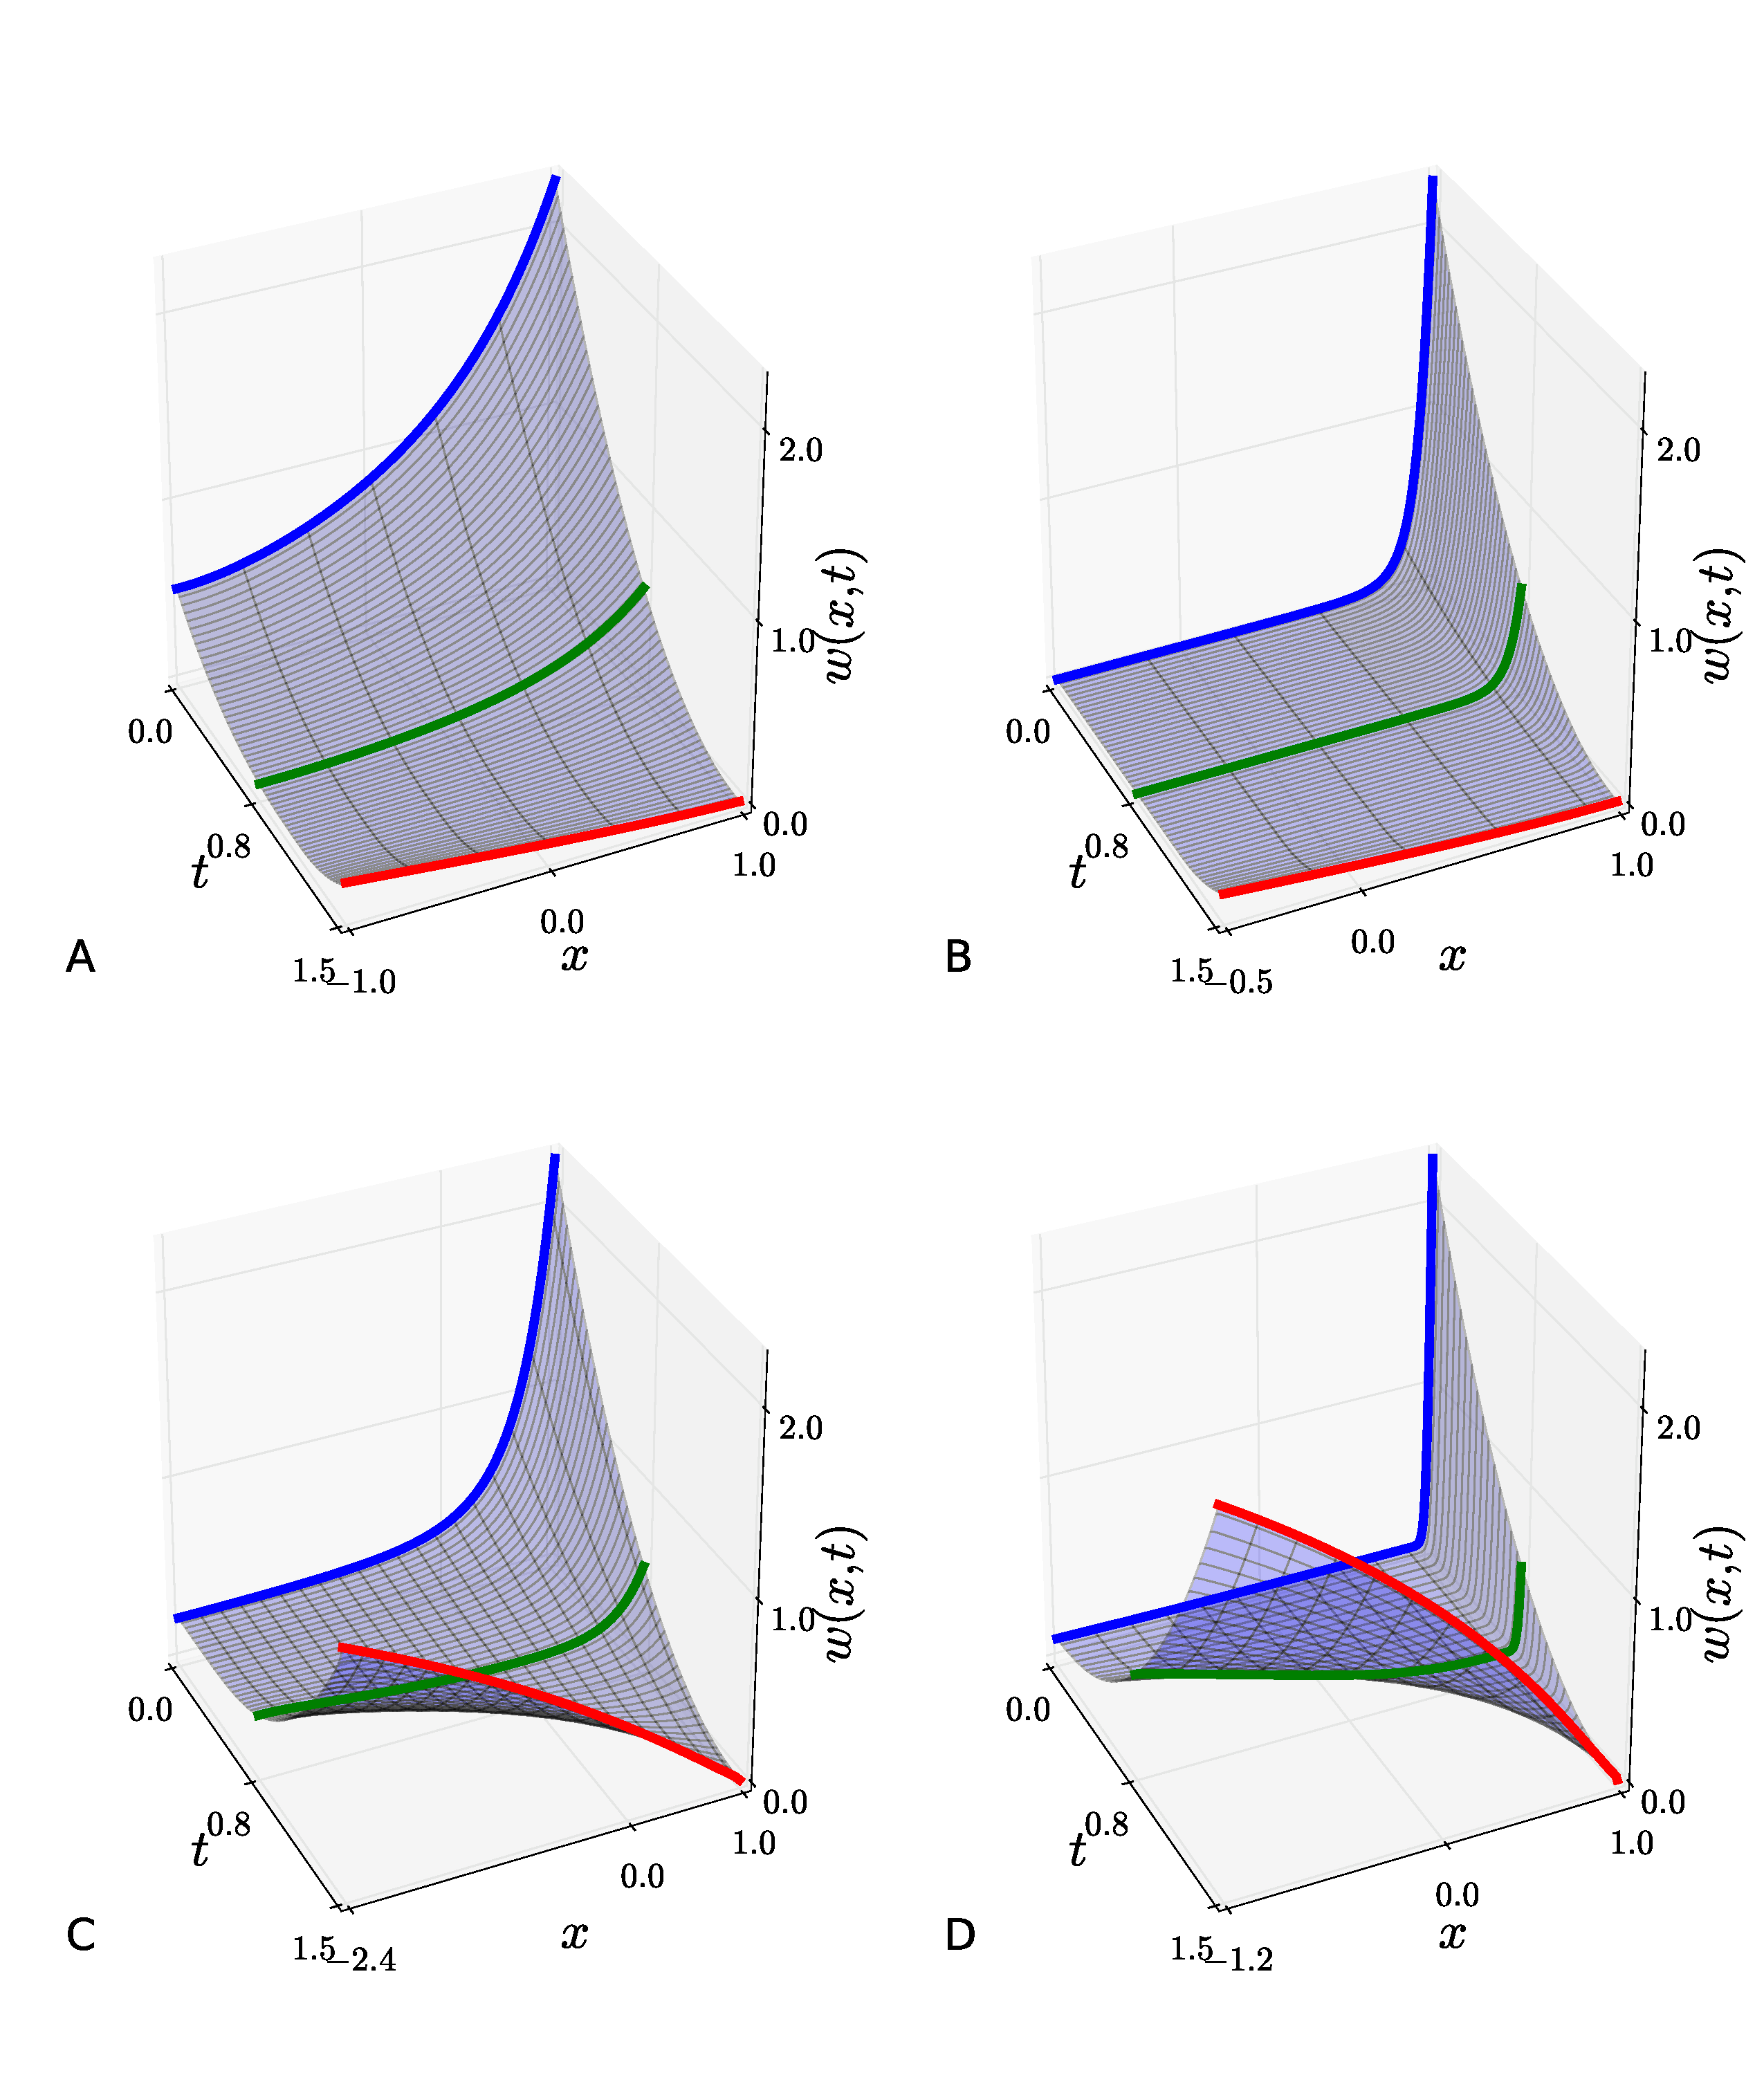
\includegraphics[width=0.99\textwidth]{Figs/HJB/Regimes_valuesurf.pdf}
\caption{The numerical solution for the value function $\v(x,t)$ HJB PDE,
\cref{eq:OC_LS_HJB_full}, for the four different parameter regimes.
The desired spike time is set to $\T=1.5$.
The control bounds are $\a \in [-2,2]$. 
The coloured contours for fixed $t$ plotted in thick correspond to the
curves plotted in the left panels of \cref{fig:HJB_4regimes_value_control_cuts}
(blue: $t=0$, green: $t=t*/2$, red: $t=t*$).
\\
A) Supra-Threshold-Low-Noise
B) Supra-Threshold-High-Noise
C) Sub-Threshold-Low-Noise 
D) Sub-Threshold-High-Noise  }
\label{fig:HJB_4regimes_value_surf}
\end{center}
\end{figure}

Let us discuss the most salient features in
\cref{fig:HJB_4regimes_value_surf,fig:HJB_4regimes_value_control_cuts}. Recall
that lower values for the value function, $\v(x,t)$, are preferred, since we are
minimizing. We see the same general shape in all four space-time surface plots
of the value function in \cref{fig:HJB_4regimes_value_surf}. At the end of the
interval, $\v(x,\T)$ is monotonically decreasing in $x$, which is to be expected
given its terminal condition in \cref{eq:valuefun_TCs}. That is, the lower the
value of $X(\T)$ the more on average will we have to wait for the spike to
occur.
% This same basic shape represents the idea that we would like to be close to
% the threshold, $x = 1$, near the end of the interval when $t \approx \T$, but
% we would like to be far from threshold, for $t \ll \T$. Indeed, at the very
% end of the interval, when $t = \T$, the value function, $v(x,\T)$, is
% monotonically decreasing in $x$, because the lower the value of $X_\T$ the
% more time on average will it take us to spike and the more delay will we have
% from our desired spike time.
As we go back in time $\v$ inverts, with a clear peak near the upper, threshold
boundary. That is, for intermediate values of $t$ we have to consider the risk
of spiking too early, represented by the high value of $\v$ near the upper
boundary {\sl and} the risk of spiking too late, represented by the high values
of $\v$ at the lower boundary. As we progress even further back in time to the
beginning of the interval, the peak near the threshold rises further, since we are spiking
{\sl earlier}, while the peak at the lower end flattens, since now there is
enough time to reach threshold despite starting far from it. The full surface
plots for $\v(x,t)$ in \cref{fig:HJB_4regimes_value_surf} can be thought of as
the interpolation between these three basic phases.

% Note, that exact shape is generated by Since we have put a very small weight
% on the energy penalty, $\e = .001$, and we have a significantly high bound on
% the maximum / minimum of the applied control, the value function becomes quite
% flat for $x \ll 1$ and $t \ll \T$, since it is likely that we can apply enough
% control to avoid an early spike and still drive the system close to threshold
% at the desired time, $t = \T$
Now focus on the controls, on the right in
\cref{fig:HJB_4regimes_value_control_cuts}. Naturally, at the end of the
interval, the control takes its maximum value, $\a(x,\T) = \amax$ for all $x$,
i.e.\ it gives the maximum available push for the neuron to spike. This is
consistent with \cref{eq:valuefun_TCs}. As we go back in time,
however, the control $\a$ decreases for $x \ll \xth$, and it becomes negative, i.e.\ inhibitory for $x
\lesssim \xth$. That is intuitively consistent with the problem objective. 
For $t<\T$, we want to bring $X(t)$ closer to the threshold, but not too close, to
avoid early spiking. 

Now consider the differences between the individual regimes, i.e.\ the
effect of changing the bias and the noise intensity, $\m,\b$. All things being
equal, the effect of increasing the noise intensity, $\b$, is to lift the value
function, i.e.\ to make our objective worse, at the beginning of the interval
and to decrease it at the end. This is to be expected since we are attempting to
minimize the variance in the spike time and without noise there would be no
variance at all. However, at the end of the interval, noise only helps, since
now we are only interested in spiking as soon as possible, and a higher noise
intensity will tend to decrease the spike time on average. Increasing $\b$ also
has the effect of increasing the size of the boundary layer near $\xth$, where
the value function rises steeply. I.e.\ for small $\b$ that layer is small since
the risk of spiking early is only significant close to the threshold. For larger
$\b$ this layer increases, see panels A,C, with a thin layer, vs.\ B,D, with a
thicker layer, in \cref{fig:HJB_4regimes_value_control_cuts}. Similarly,
increasing the bias, $\mu$, tends to decrease the value function, especially at
the end since that has the unequivocal effect of preventing late spikes.
 
 
\section{Open-loop Stochastic Control}
When the value of $X(t)$ is unobservable, the transition density can be used to
perform the optimization. Since the transition density follows a deterministic
PDE, we apply a Maximum Principle for PDEs as a method of obtaining the optimal
control, see \cite{Borzi2012} for details on optimization with PDEs, or the
article, \cite{Annunziato2010}, for optimization with a
Fokker-Planck-type of system.

\subsection{Fokker-Planck equation for the state density evolution}
We write the transition density of $X$, conditional on no
spikes having occurred since $t=0$ as:
\begin{align*}
f(x,t) \intd{x} &= \Prob[X(t)\in \intd{x} \,\big|\, X(0) = 0,\, X(s) < \xth
\quad \forall s < t].
\end{align*}
Then $f$ satisfies a Fokker-Planck equation with absorbing boundaries,
see Ch.\ 7 in \cite{Jacobs},
\begin{equation}
\begin{gathered}
\di_t f(x,t) =
				\frac{\b^2 }{2}\cdot \di^2_x f -
				\di_x \Big[ \left( \m + \a(t)- \frac{x}{\tc}\right)  \cdot f \Big].
\\
\\
\begin{array}{ll}
	& 
	\left\{ \begin{array}{lcl}
	 f(x,0) &=& \delta(x) \quad \textrm{delta function}
	\\
	(\m + \a(t)- \tfrac x \tc)f - \di_x \tfrac {\b^2}2 f] \big|_{x=\xmin} &\equiv&
	0 \quad \textrm{reflecting BCs at some } \xmin
	\\
	f(x,t) |_{x=\xth} &\equiv& 0 \quad \textrm{absorbing BCs at } \xth
\end{array} \right.
\end{array}
\label{eq:FP_pde_OU_PDF}
\end{gathered}
\end{equation}
In theory, $\xmin = -\infty$, but in the numerics below we will need to
truncate it to some finite value, exactly as in the HJB equation,
\cref{eq:OC_LS_HJB_full}.
Note that we write $\a(t)$ here instead of $\a(x,t)$ since we cannot use the
value of $X(t)$.

The $f$ dynamics can also be written as
$$
\di_t f(x,t) = - \di_x \phi(x,t)
$$
for the probability flux
$$
\phi(x,t) = (\m + \a(t) - \tfrac x \tc)f - \di_x [\tfrac {\b^2}2 f].
$$
Then the lower BC is
$$
\phi(x,t) |_{x=\xmin} \equiv 0.
$$

We will also need a short hand notation for the differential operator on the
right side of \cref{eq:FP_pde_OU_PDF}. Let
$$ \L_\a[\cdot] := \di^2_x \Big[\frac{\b^2 }{2} \cdot\Big] -
 \di_x \Big[ (\m + \a(t)- \frac{x}{\tc}) \cdot \Big],$$
 where
 $[\cdot]$ indicates the argument of the operator $\L_\a$. We will usually
 omit the subscript $\a$, but have written it now to emphasize that the
 differential operator is parametrized by the control, $\a$.

\subsection{Restating the objective in terms of the transition density}
We now derive the optimality conditions for the optimal control $\a^*$ for the
open-loop context. Recall our objective, \cref{eq:OC_LS_variance}.  
% $$
% J[\a(\cdot)] = \Exp\left[
% (\ts - \T \big)^2
% +
% \e \int_0^\ts  \a^2(s) \intd{s}
% \right].
% $$
We can write this in terms of the transition density, $f$, as:
\begin{align}
J[\a(\cdot)] =&
\int_\xmin^\xth \Ttwo(x) \cdot f(x,\T) \intd{x}
\notag
\\
&+ \int_0^\T \phi(\xth, t) (t-\T)^2 \intd{t}
\label{eq:OC_LS_variance_density}
\\
&+  \e \int_0^\ts  \a^2(t)  \cdot \left(  \int_\xmin^\xth f(x,t) \intd{x}
\right)
\intd{t}.
\notag
\end{align}
Let us explain in more detail each term on the right-hand side in
\cref{eq:OC_LS_variance_density}.

The first term, $$ \int_\xmin^\xth \Ttwo(x) \cdot f(x,\T)\intd{x}, $$ counts the
cost of trajectories which spike too late. This cost is the expected squared time-to-hit starting at $x$, with  $\a = \amax$, weighted by the
probability of $X(\T) = x$, which is just $f(x,\T)$. Recall that $\Ttwo$ is
defined in \cref{eq:Trem_squared}.

The second term, $$ \int_0^\T \phi(\xth,t) (t-\T)^2 \intd{t}, $$ counts the cost
of trajectories which spike too early, that is the squared difference between
some realized spike time, $\ts = t$, and desired spike time $\T$, weighted by
the probability of a spike at $t$ which is just the outward probability flux at
the threshold, $\phi(\xth,t)$. Recall that we assume that $\xth = 1$ throughout.
Note further that due to the homogeneous Dirichlet BC at $\xth$, $f(\xth) = 0$, the outward flux is simply $$ \phi(\xth, t) = -\frac{\b^2 }{2} \di_x f(\xth,
t).$$

Finally, the third term,
$$
\e \int_0^\ts  \a^2(t)  \cdot \left(  \int_\xmin^\xth f(x,t) \intd{x} \right)
\intd{t}, $$
is the energy cost; the inner integral, $\int_\xmin^\xth f(x,t) \intd{x}$,
takes into account that we incur an energy cost only for those trajectories
which have not yet spiked.

With that our optimal control $\a^*(\cdot)$ will naturally be found via:
$$
\a^*(\cdot) = \argmin_{\a(\cdot)} J[\a(\cdot)].
$$

\subsection{Optimizing using a Maximum Principle}
\label{sec:PDE_max_principle_for_pdf}
By now our stochastic optimal control problem modelled by SDEs
has become a deterministic optimal control problem modelled by PDEs. Our control
$\a$ influences the evolution density $f$ and via $f$, the integrals in the
objective, $J$.

The Maximum Principle for PDEs, which is an extension to the famous Pontryagin
Maximum Principle from finite dimensional systems, introduces an adjoint
variable, $p$, which solves a PDE related to the PDE satisfied by the density
$f$ and then calculates the optimal control, $\a(\cdot)$, as a functional of $f$
and $p$.

In short, the equation for the adjoint function, $p$, is
\begin{equation}
\begin{gathered}
\begin{aligned}
\di_t p =& - \Lstar[p]
\\
		=&
			- \Big[ \frac{\b^2 }{2}\cdot \di^2_x p +
			(\m + \a(t)- \frac{x}{\tc})  \cdot \di_x p \Big].
\end{aligned}
\\
\begin{cases}
	p \big|_{x=\xth} &= (t-\T)^2
	\\
	\di_x p  \big|_{x=\xmin} &= 0
	\\
	p(x,\T) &= \Ttwo(x)
\end{cases}
\label{eq:adjoint_pde_OU}
\end{gathered}
\end{equation}

and then $\a$ can be found via
\begin{equation}
\Big\{
 \e 2 \a(t)
+ p f \Big|_\xmin
- \int _\xmin^\xth p \cdot \di_x f \intd{x}
\Big\} = 0
\quad \forall t \in [0,T].
\label{eq:J_necessary_condition}
\end{equation}
Roughly speaking, \cref{eq:J_necessary_condition} corresponds to setting the
derivative of the objective $J$  with
respect to $\a$ to zero, in \cref{eq:OC_LS_variance_density} and the
adjoint state $p$ acts as a Lagrange multiplier corresponding to the constraints of
the transition density dynamics.

More practically, the quantity

\begin{equation}
\delta_\a J (t) =  \Big\{
- \int _\xmin^\xth p(x,t) \cdot \di_x f(x,t) \intd{x}
+ p(x,t) f(x,t) \Big|_\xmin
+ \e  2 \a(t)
\Big\}
\label{eq:hamiltonian_gradient}
\end{equation}
gives the direction of increase of $J$ at $\a(t)$
and we can use it as a gradient in a descent algorithm, given some initial
guess, $\a_0(t)$, for the control.

Finally, we are ready to calculate the open-loop stochastic optimal control for
the four parameter regimes. We use the same numerical method for solving the
PDEs as described in \cref{sec:hjb_numerix}, since the PDEs for $f,p$ are very
similar in structure to the PDE for $\v$ except they do not contain a nonlinear
term. The details of the simple gradient descent algorithm for obtaining the
optimal open-loop control are given in algorithm
\ref{alg:gradient_descent_4_OC}. See \cite{Annunziato2013} for a more
sophisticated descent method based on the conjugate-gradient method. For our
applications, the algorithm in \ref{alg:gradient_descent_4_OC} typically
converges in less than 10 iterations, although sometimes it can take longer. 
\begin{algorithm}
\begin{algorithmic}
\State Fix $\T, \e, \ldots$ the problem parameters
\State Fix $\{t_n\}_0^{N_t}$ a time-discretization of $[0,\T]$
\State Fix $g_{tol}$ a convergence tolerance for the gradient
\State Fix $K_{\max}, J_{\max}$ number of maximum iterations in outer, resp.
inner descent loops
\State Fix $s$ the initial step-size. 
\\ {\itshape $\#$ we use $g_{tol}=1e-5,K_{\max}=100,J_{\max}=10,s=10$}
\State $\a_1(t) \gets (\amax-\amin) \cdot t / \T + \amin$ 
\\{\itshape  $\#$ $\a_1(t) \sim$ initial guess for the control, linear
interpolate between $\amin, \amax$}
\For { $k= 1\dots K_{\max}$} 
\\ {\itshape $\#$ This is the outer loop where we descend down different
gradients}
 \State Calculate $f_k,J_{k},p_k, \delta_\a J_k$ corresponding to
	$\a_k$ from
	\cref{eq:hamiltonian_gradient,eq:adjoint_pde_OU,eq:FP_pde_OU_PDF,eq:OC_LS_variance_density}
	\State $N_{active}\gets$   Number of time nodes $t_n$, where either
	$\a_k(t_n) \neq \{\amin, \amax\}$ or $\delta_\a J_k(t_n)$ points inwards
	\If{ $|| \delta_\a J_k||_{\R^{N_{active}}} \leq g_{tol}\cdot N_{active}$}
		  \\ {\itshape  $\#$ 'Active' gradient is small enough,
		 consider converged:}
		 \State BREAK
	\EndIf
	\\ {\itshape $\#$ Find the step size, $s$, of how far to move $\a$ in the
	direction $\delta_\a J_k$:}
	\For { $j= 1\dots K_{\max}$}
	\\ {\itshape $\#$ This is the inner loop where we find how much to descend down
	the current gradient}
	\State $\a_{k,j} \gets \a_{k} - s_j \cdot \delta_\a J_k  $
	\\ {\itshape $\#$ $\a_{k,j}$ is the new control strategy to try}
	\State Calculate $f_{k,j}, J_{k,j}$ corresponding to
		$\a_{k,j}$ from	\cref{eq:FP_pde_OU_PDF,eq:OC_LS_variance_density}
	\\ {\itshape $\#$ Recall $f_{k,j}$ is a probability density resulting from the
	control $a_{k,j}$ and $J_{k,j}$ is the objective value resulting from
	$f_{k,j}$}
	\If {$J_{k,j} < J_k$}
		\\ {\itshape $\#$ We found a better (smaller) objective value}
		\State $s \gets 2 s_j$ {\itshape $\#$ try a more aggressive step in the
		next iteration}
		\State BREAK
		\EndIf
	\If {$j == J_{\max}$}
		\\ {\itshape $\#$ We exhausted the step search without finding a 
		smaller $J$, return current values}
		\State Return $J_k, \a_k$
	\EndIf
 	\\ {\itshape  $ \#$ Continue the inner looop, now try with a smaller step:}
	 	\State $s_{j+1}$ \gets $s_j / 2.$
    \EndFor  {\itshape $\quad \#$ single step loop}
	\If {$k == K_{\max}$}
		\State ERROR 'Could not converge'
	\EndIf
    \\{\itshape $\#$ Assign the new candidate for the optimal control and
    re-loop}
		\State $\a_{k+1} \gets \a_{k,j}$
\EndFor {\itshape $\quad \#$ gradient descent loop}
\State \Return $J_k, \a_k$
\end{algorithmic}
\caption{ Gradient descent algorithm for obtaining the optimal open-loop 
control}
\label{alg:gradient_descent_4_OC}
\end{algorithm}

The optimal controls obtained using algorithm \ref{alg:gradient_descent_4_OC} for each regime are in
\cref{fig:FBK_Regimes_cs}. Recall that the optimal control, $\a^*(t)$, is open-loop and thus it is only a function of time.
% \usepackage{graphics} is needed for \includegraphics
\begin{figure}[htp]
\begin{center}
%   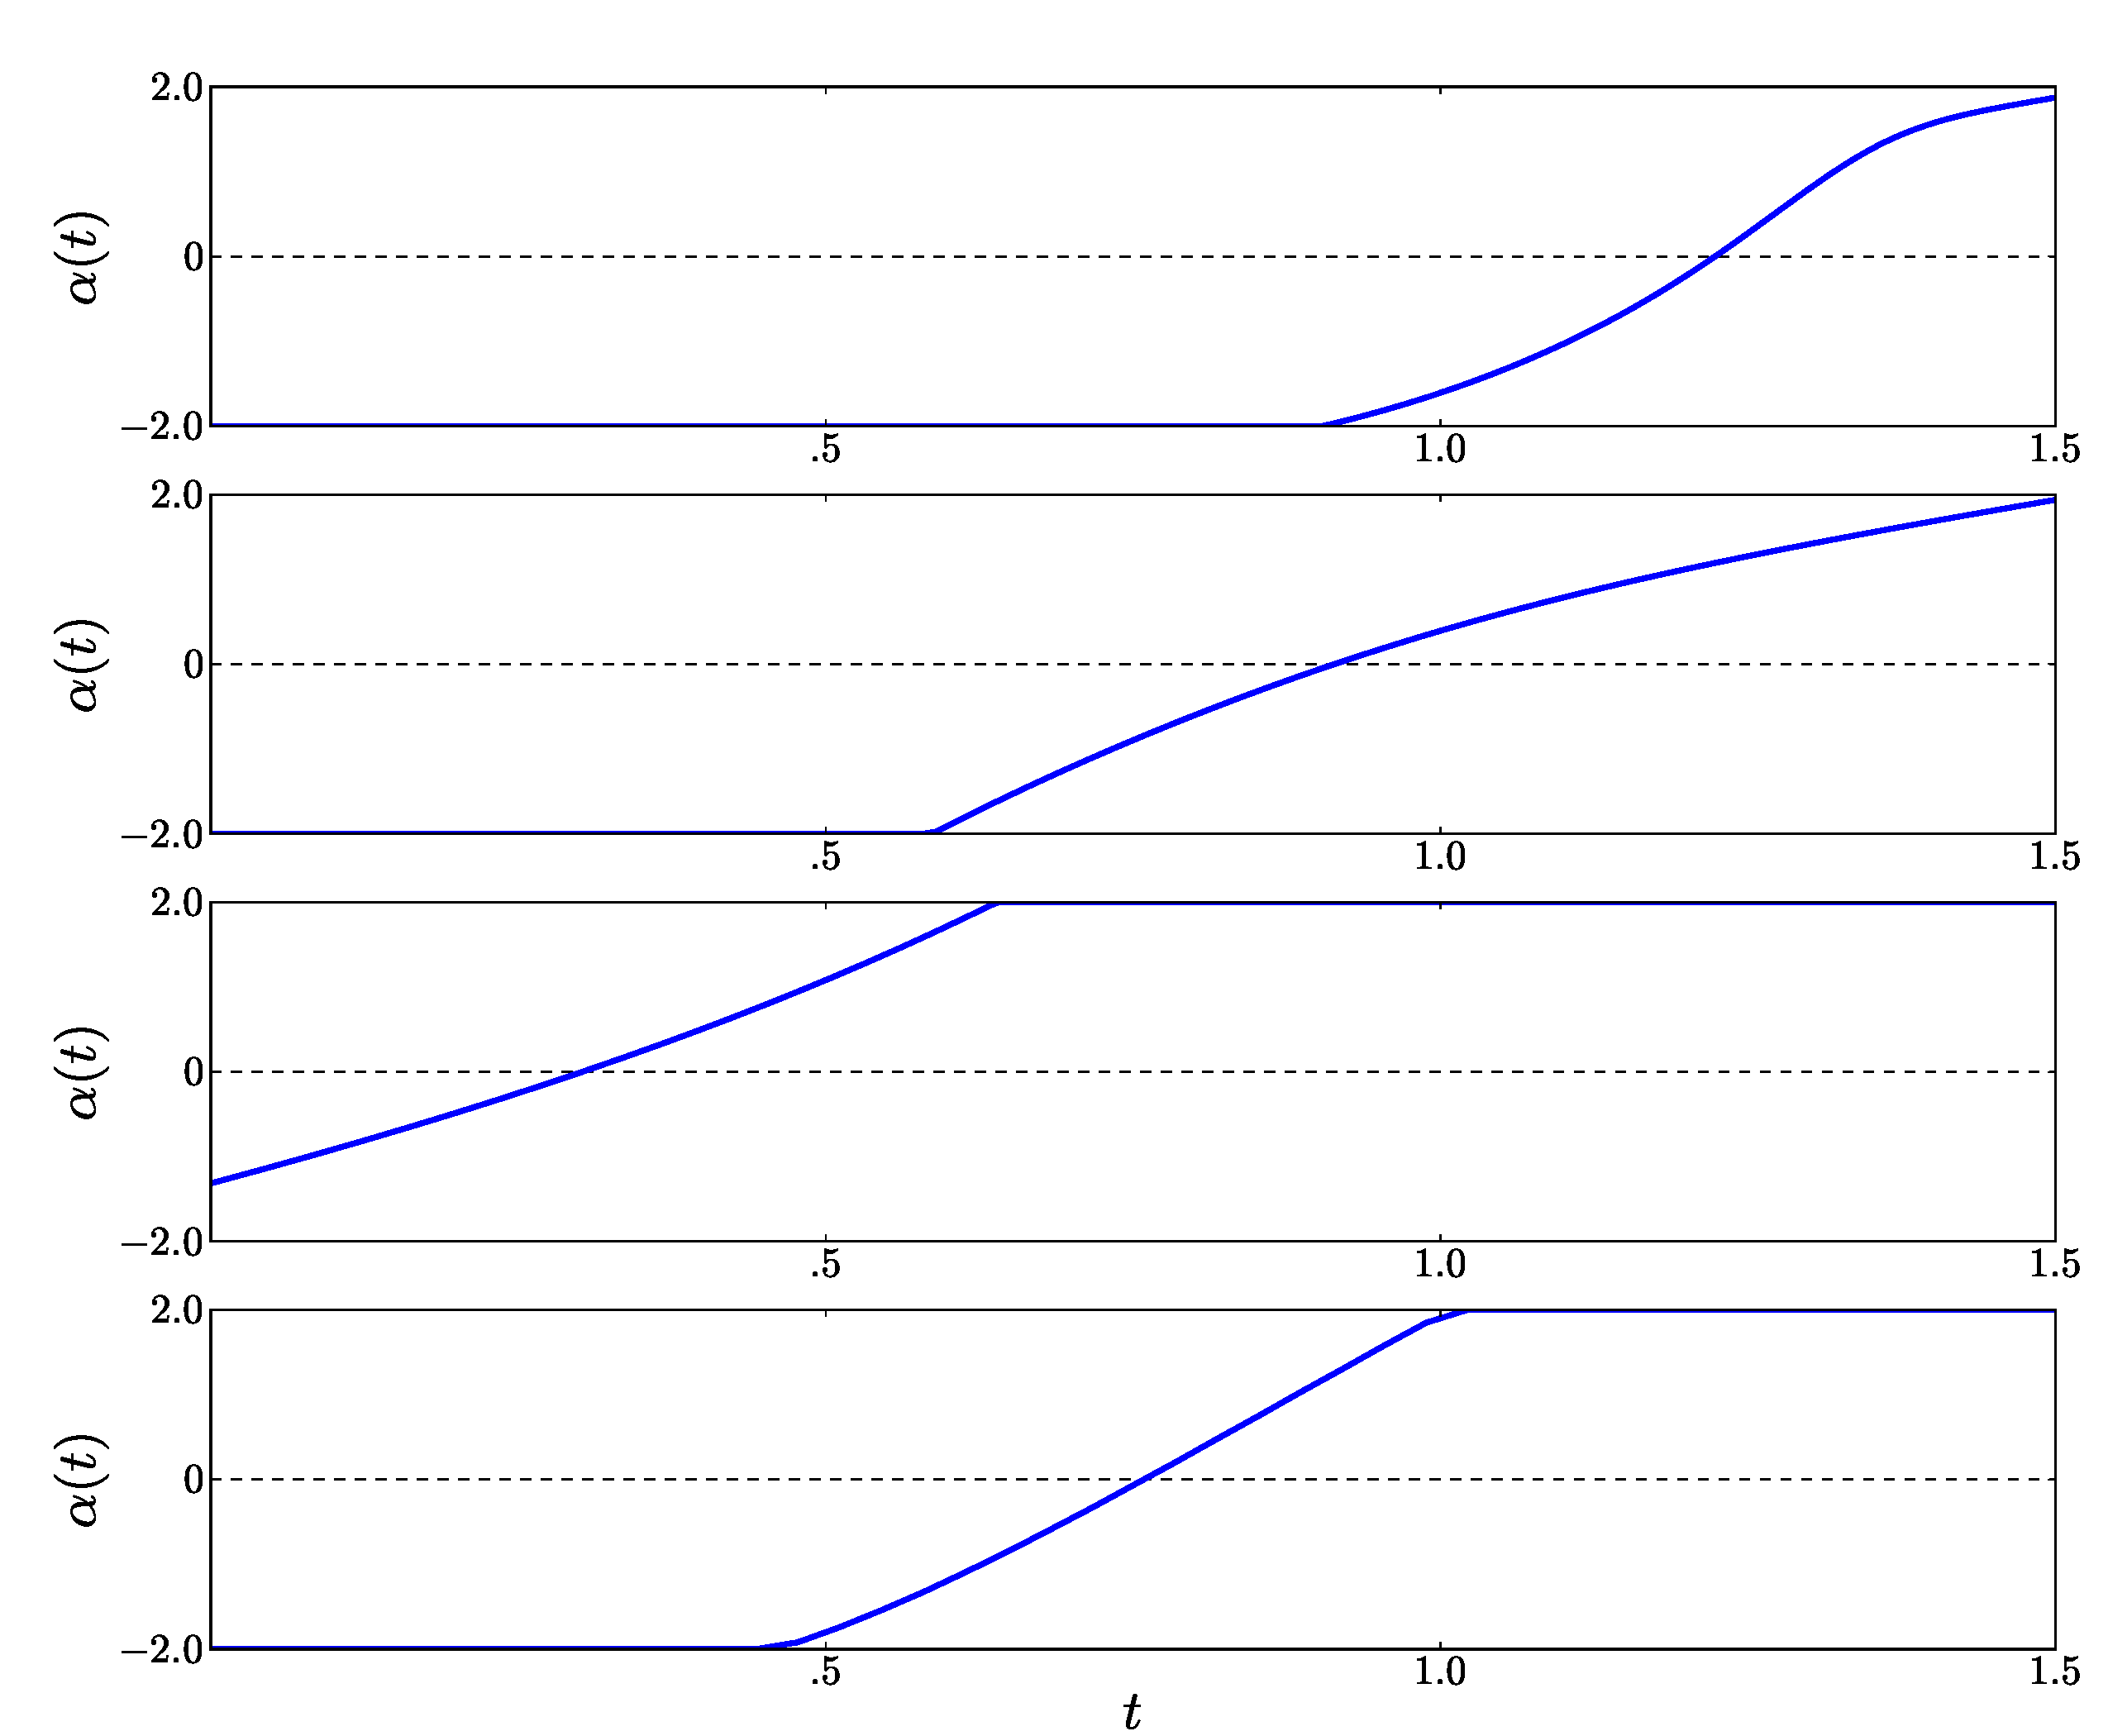
\includegraphics[width=\textwidth]{Figs/FP_Adjoint/Regimes_cs.pdf}
  \includegraphics[width=\textwidth]{Figs/FP_Adjoint/Regimes_cs_singleplot.pdf}
  \caption[labelInTOC]{The deterministic optimal controls for each parameter
  regime as functions of time, $t \in [0, \T]$.
  The desired spike time is set to $\T=1.5$, the energy penalty, $\eps
  = 0.001$ and the bounds are $\a \in [-2,2]$.
  From left-to-right, the control curves correspond to the
  Sub-Threshold-Low-Noise, Sub-Threshold-High-Noise, Super-Threshold-High-Noise,
  Sub-Threshold-Low-Noise regimes
%   A) Supra-Threshold-Low-Noise 
%   B) Supra-Threshold-High-Noise
%   C) Sub-Threshold-Low-Noise
%   D) Sub-Threshold-High-Noise  
  }
  \label{fig:FBK_Regimes_cs}
\end{center}  
\end{figure}   

Let us discuss the most salient features of the controls calculated in
\cref{fig:FBK_Regimes_cs}. In general, the strategy is to inhibit the neuron at
the beginning of the interval, $\a(t) = \amin$ for $t \ll \T$ and to excite it
near the end, $\a(t) = \amax$ for $t \approx \T$. The smooth portion that
connects these two segments in the middle of the interval is due to the energy
penalty, $\e \int \a^2(s) \intd{s}$. The behaviour of the control in different
regimes is relatively simple to explain and we see what we would expect. In a
sense the bias current $\mu$ can be absorbed by the control and so increasing
$\mu$ amounts to decreasing $\a$ modulo its bounds. That is exactly the
difference between the Super-Threshold vs.\ Sub-Threshold plots in
\cref{fig:FBK_Regimes_cs} when holding the noise intensity fixed, either
$\b=0.3$ or $\b=1.5$. Both for low and high noise intensity, a reduction of $\mu$
results in an increase in $\a(t)$. 
The effect of varying the noise intensity, $\b$, is more subtle and it is not
the same in the Supra vs.\ the Sub-Threshold regimes. In the
Supra-Threshold regime, reducing $\b$ reduces the need for
excitatory control towards the end, since the bias alone should put the neuron
over the threshold. Thus the main part of the control with low noise in the
Supra-Threshold regime is to stop the neuron from spiking too early. In the
Sub-Threshold regime, the situation is somewhat reversed - reducing
$\b$ obviates the need to apply an inhibitory control in the early part of the
interval and also prompts the controller to apply excitatory input earlier,
since it is the controller which is now the main drive for a spike.

% An example for . The results are in
% \cref{fig:FP_adjoint_objective_control_convergence}.
% \begin{figure}[h]
% \begin{center}
% \subfloat[$\a_k(t)$ ]
% {
% \includegraphics[width=0.48\textwidth]
% {Figs/FP_Adjoint/ExampleControlConvergence_control.png}
% }
% \subfloat[$J_k$ ]
% {
% \includegraphics[width=0.48\textwidth]
% {Figs/FP_Adjoint/ExampleControlConvergence_objective.png}
% }
% \caption[ ]{The result of an entire optimization iteration, on the left the
% iterates of the control, $\a_k(t)$, on the right the progress of the
% objective with each iteration. The final control, in purple, is inhibitory at
% the beginning of the time interval, $\a < 0$, unlike the the deterministic
% control solution.
% We see a significant
% reduction in the objective value, $J$, and thus an improvement, on the
% order of 50\%.}
% \label{fig:FP_adjoint_objective_control_convergence}
% \end{center}
% \end{figure}
%
% \begin{table}[h]
% \centering
% \begin{tabular}{lc}
% Control Law & Squared Error \\
% \hline
% Deterministic &  0.647 \\
% Stochastic &  0.336\\
% Theory (Value function) & 0.285
% \end{tabular}
% \caption{Realized performance of the different control laws and the theoretical
% expected performance of the stochastic law (last row)}
% \label{tab:realized_avg_errors_det_vs_stoch}
% \end{table}
%
% \begin{figure}[h]
% \begin{center}
% \subfloat[A]
% {
% \label{fig:controlled_traj_ex1}
% \includegraphics[width=0.33\textwidth]
% {Figs/ControlSimulator/example_controlled_trajectories_id1.png}
% }
% \subfloat[B]
% {
% \label{fig:controlled_traj_ex2}
% \includegraphics[width=0.33\textwidth]
% {Figs/ControlSimulator/example_controlled_trajectories_id4.png}
% }
% \subfloat[C]
% {
% \label{fig:controlled_traj_ex3}
% \includegraphics[width=0.33\textwidth]
% {Figs/ControlSimulator/example_controlled_trajectories_id3.png}
% }
% \caption[]{Examples for the controlled trajectories using both the deterministic
% and the stochastic control approaches. The red vertical line in the plots
% indicates the desired spike-time, $\T$. In A, B the performance of both
% control laws is essentially the same, but in C we see the advantage of the
% stochastic approach. $\tc, \b = [.75, 1.25]$.}
% \label{fig:control_trajectories_examples}
% \end{center}
% \end{figure}
% \begin{figure}[htp]
% \begin{center}
%   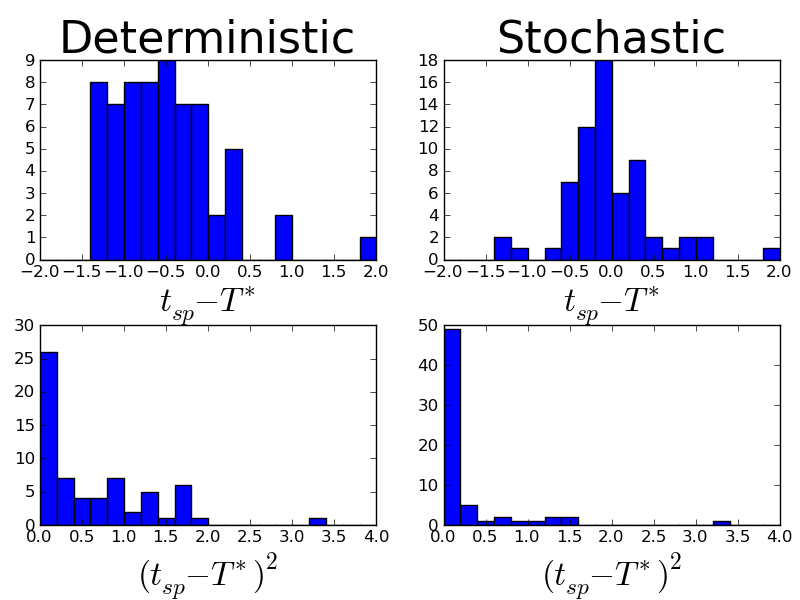
\includegraphics[width=.9\textwidth]{Figs/ControlSimulator/example_controlled_trajectories_hists.png}
%   \caption[labelInTOC]{Histogram of the spike timing error for the
%   deterministic (left) vs. the stochastic (right) control laws.}
%   \label{fig:error_histograms_det_vs_stoch}
% \end{center}
% \end{figure}

\section{Simulations} 
\subsection{Single-Spike Control}
\label{sec:probabilistic_numerical_test}
Having obtained the optimal controllers, both closed- and open-loop, we evaluate
their performance with simulated realizations of the voltage process,
\cref{eq:X_evolution_uo}. In particular, while they both minimize the expected
squared deviation of the spike-time from some desired spike time, we analyze
the distribution of the squared deviation and the behaviour of the
controls for different parameter regimes.

In addition to the optimal controllers, we also show the behaviour of
another control law - perhaps the most naive one - which is obtained by ignoring
the noise and the energy penalty. That is, we find a {\sl constant} value of
$\a$ which satisfies the desired boundary conditions, $x(0) = 0, x(\T) = \xth$. This naive
controller will be called 'Deterministic', since it assumes deterministic
dynamics in $X$, i.e.\ $\b = 0$.

For the comparison, we sample $N$ realizations of the controlled system
and apply in turn each of the three controls. Naturally, we reuse the same
realization of the underlying stochastic process, $W_t$, for each of the
three different controls.

We set $\e = 0.001$ and $\amax = 2.0$. As such the energy cost is of secondary
importance and the paramount effect on the objective is the difference $(\ts -
\T)$, which we are trying to minimize.

The performance of the three controllers for each parameter regime is given in
\cref{tab:realized_avg_errors_det_vs_openloop_vs_stoch} and
\cref{fig:error_histograms_det_vs_openloop_vs_stoch}. Naturally, the closed-loop
achieves a lower error than the open-loop, and the naive controller fares worst.
The difference in performance mostly depends on the strength of the noise. Thus,
for low noise, the performance of the stochastic controllers, be they open- or
closed-loop is not much superior to the naive deterministic controller. On the
contrary - in the high-noise regime, using a stochastic controller gives a much
lower error on average between the desired $\T$ and the realized $\ts$.

For illustration sake, we also visualize some trajectories from the
Sub-Threshold-High-Noise regime in \cref{fig:control_trajectories_examples}, see
panels A),C),E). The most notable feature of the $\a(\cdot)$ plots in
\cref{fig:control_trajectories_examples} is that especially for $\eps=0.001$,
there is a high level of fluctuations in the closed-loop $\a$. That is to be
expected from the optimality condition in
\cref{eq:OC_LS_variance_energy_quadratic_control}. Since the control is
proportional to the derivative of the value function and we are minimizing,
roughly speaking, the control attempts to push the process, $X$, to the bottom
of the valley that is formed by the value function, $\v$. However as the
stochastic fluctuations of $X(t)$ push it randomly to either side of that
'valley' and in turn force the control to change signs to counter-act.
These fluctuations are then amplified by the division by the small parameter
$\eps$ so that the control mostly bangs up or down to its extremes
$\amin, \amax$.
 
\begin{table}[h]
\begin{center}  
\subfloat[Supra-Threshold Low-Noise]{
   \input{Figs/ControlSimulator/MeanSquaredErrors__SUPT_ln.txt}}\\ 
\subfloat[Supra-Threshold High-Noise]{   
\input{Figs/ControlSimulator/MeanSquaredErrors__SUPT_HN.txt}}\\
 \subfloat[Sub-Threshold Low-Noise]{
 \input{Figs/ControlSimulator/MeanSquaredErrors__subt_ln.txt}}\\ 
 \subfloat[Sub-Threshold High-Noise]{
 \input{Figs/ControlSimulator/MeanSquaredErrors__subt_HN.txt}}\\
%  \begin{tabular}{lcc}
% Control Law &  Squared Error &  Squared Error \\
%  & Empirical & Theoretical\\% \hline 
% Deterministic &  0.621 & - \\
% Open-Loop Stochastic & 0.356 & 0.382\\
% Feedback Stochastic &  0.288& 0.285\\
% \hline % \end{tabular} - 
\caption{
Realized and theoretical performance of the different control laws. The
empirical performance is obtained using $N=10000$ sample paths. The theoretical
performance is found using the optimal value for $J$ for the open-loop
stochastic control and the value function $\v(x=0, t =0)$ for the closed-loop
stochastic control.}
\label{tab:realized_avg_errors_det_vs_openloop_vs_stoch}   
\end{center} 
\end{table} 

\begin{figure}[h]  
\begin{center}
\subfloat[Supra-Threshold Low-Noise]{
  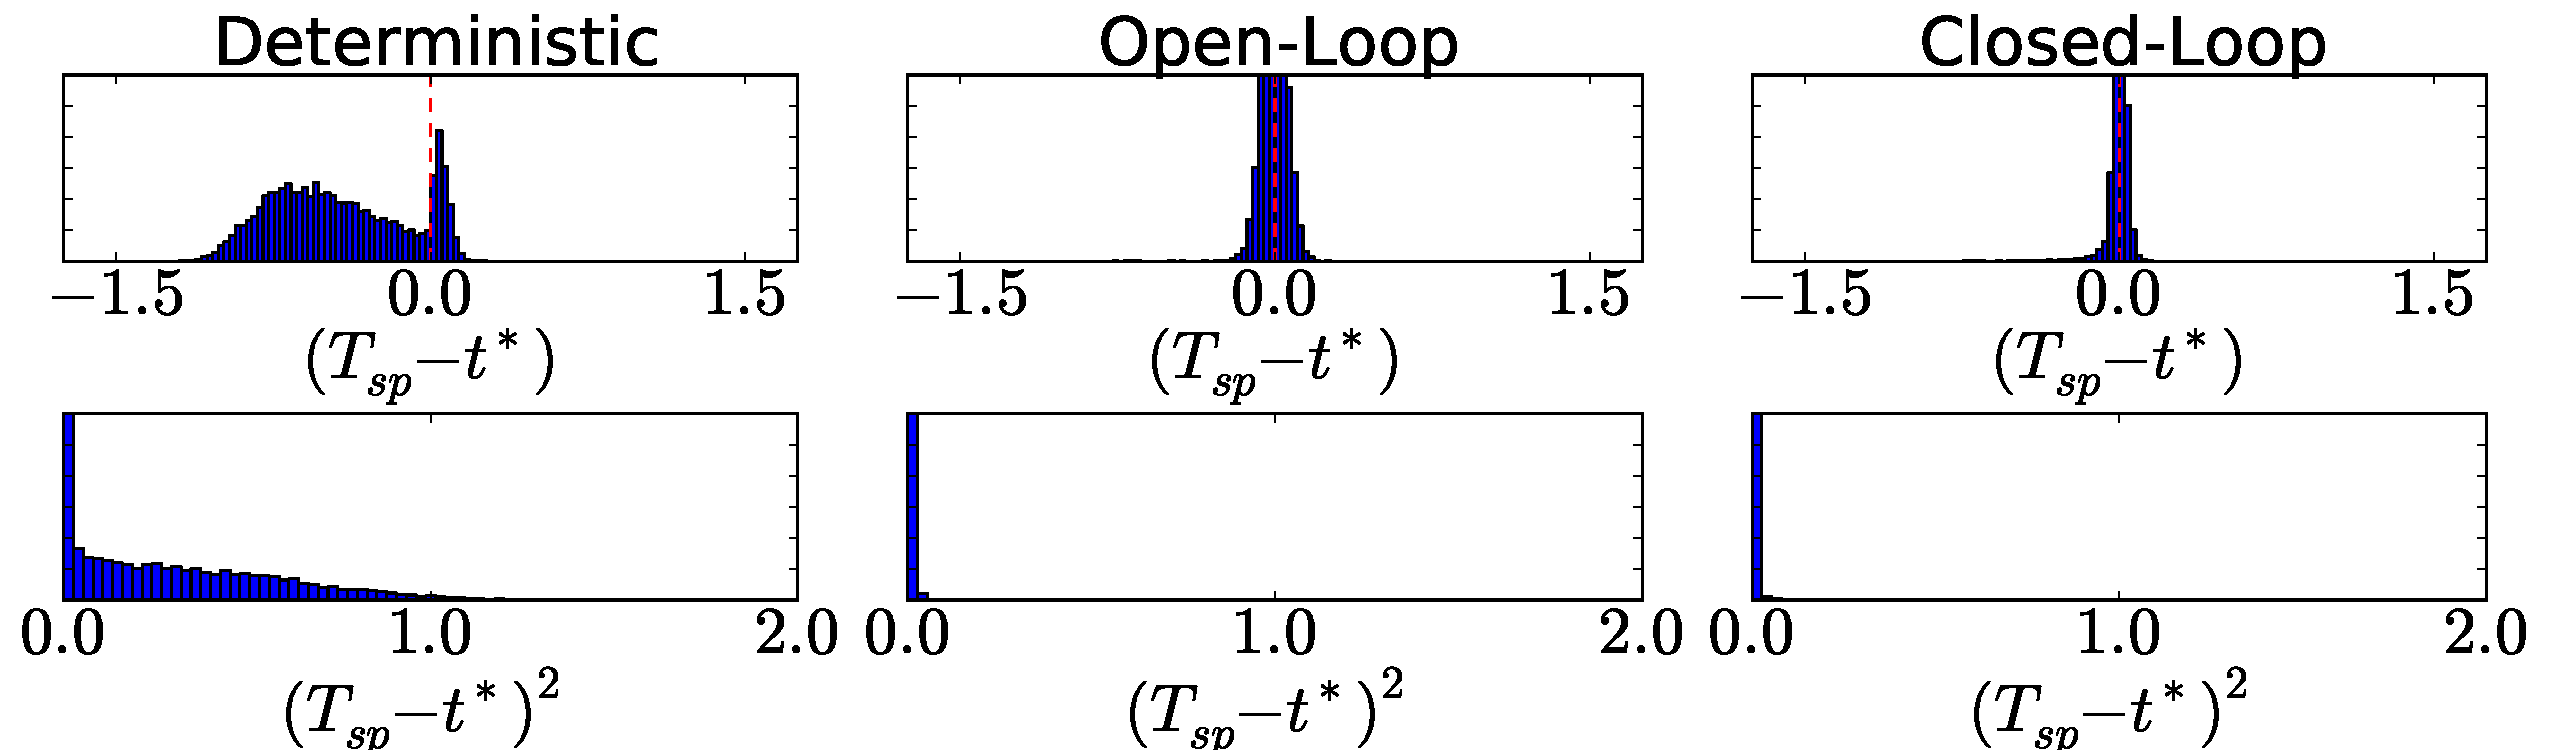
\includegraphics[width=\textwidth]
  {Figs/ControlSimulator/Regimes_SUPT_ln_errors_hist.pdf}
}
\\
\subfloat[Supra-Threshold High-Noise]{
  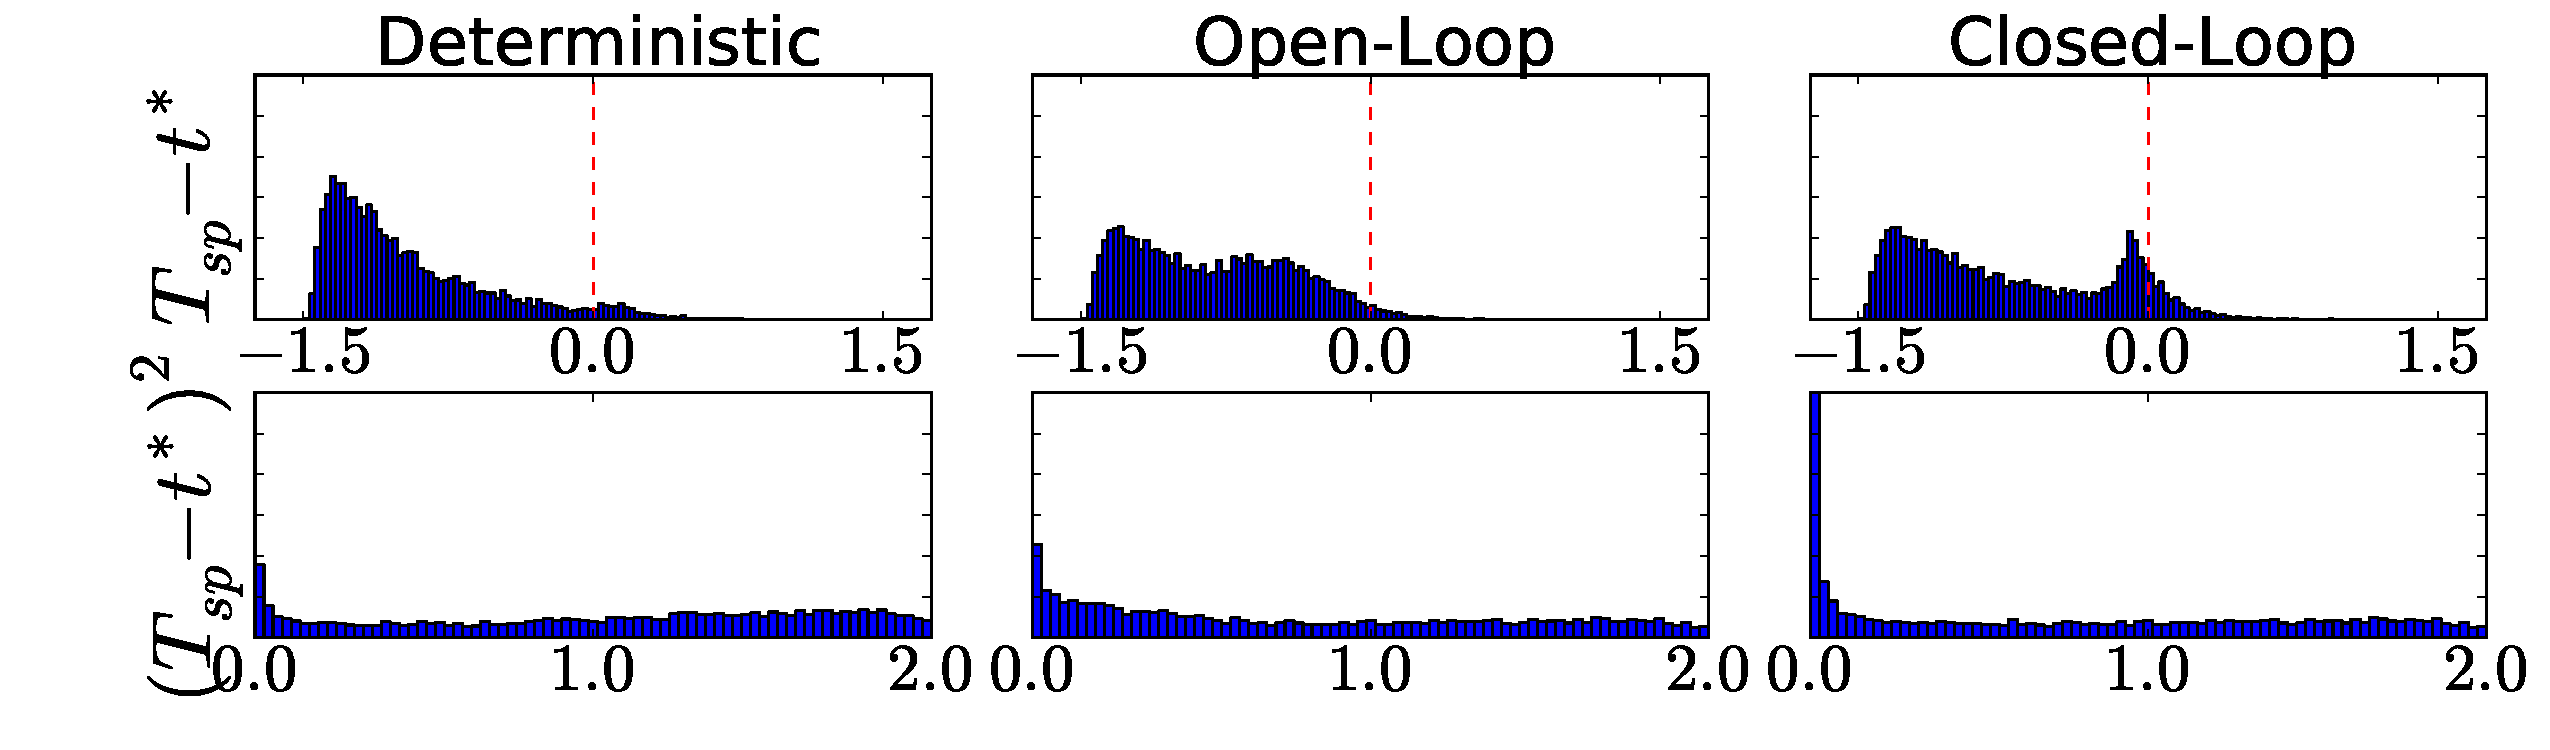
\includegraphics[width=\textwidth]
  {Figs/ControlSimulator/Regimes_SUPT_HN_errors_hist.pdf}
  }
  \\
\subfloat[Sub-Threshold Low-Noise]{
  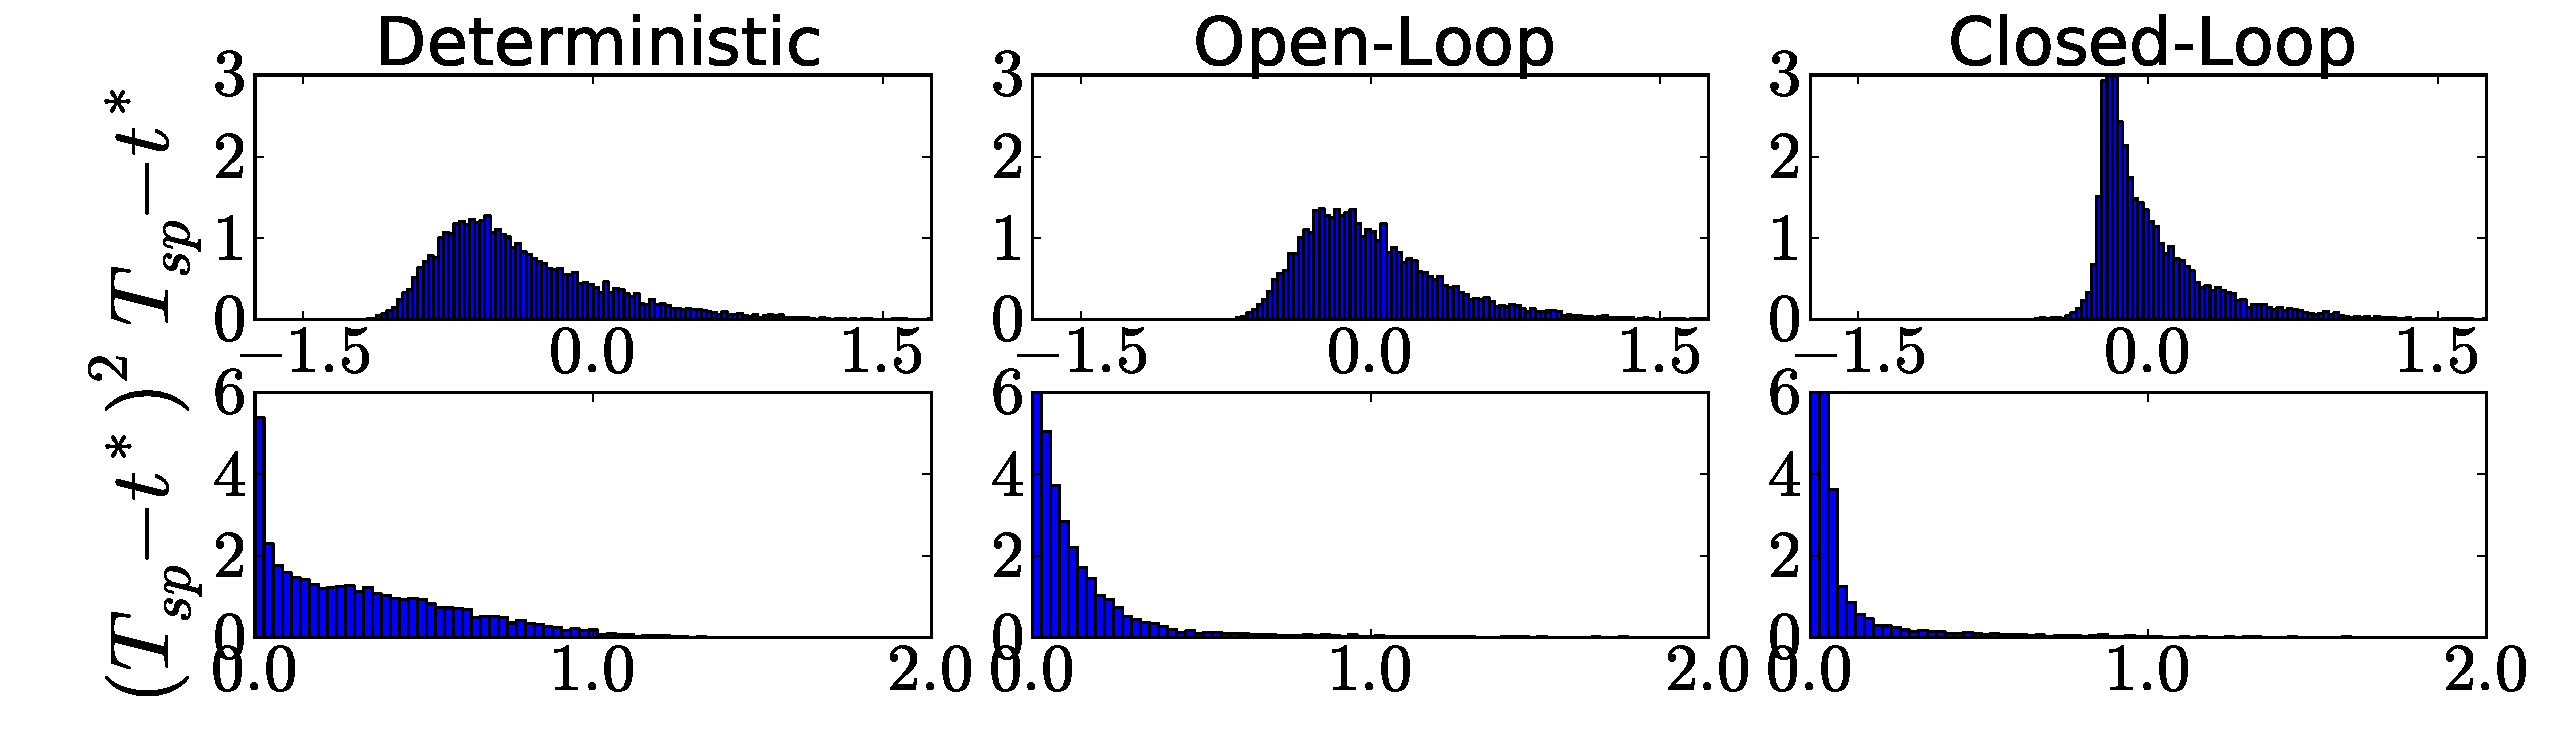
\includegraphics[width=\textwidth]
  {Figs/ControlSimulator/Regimes_subt_ln_errors_hist.pdf}
}
\\
\subfloat[Sub-Threshold High-Noise]{
  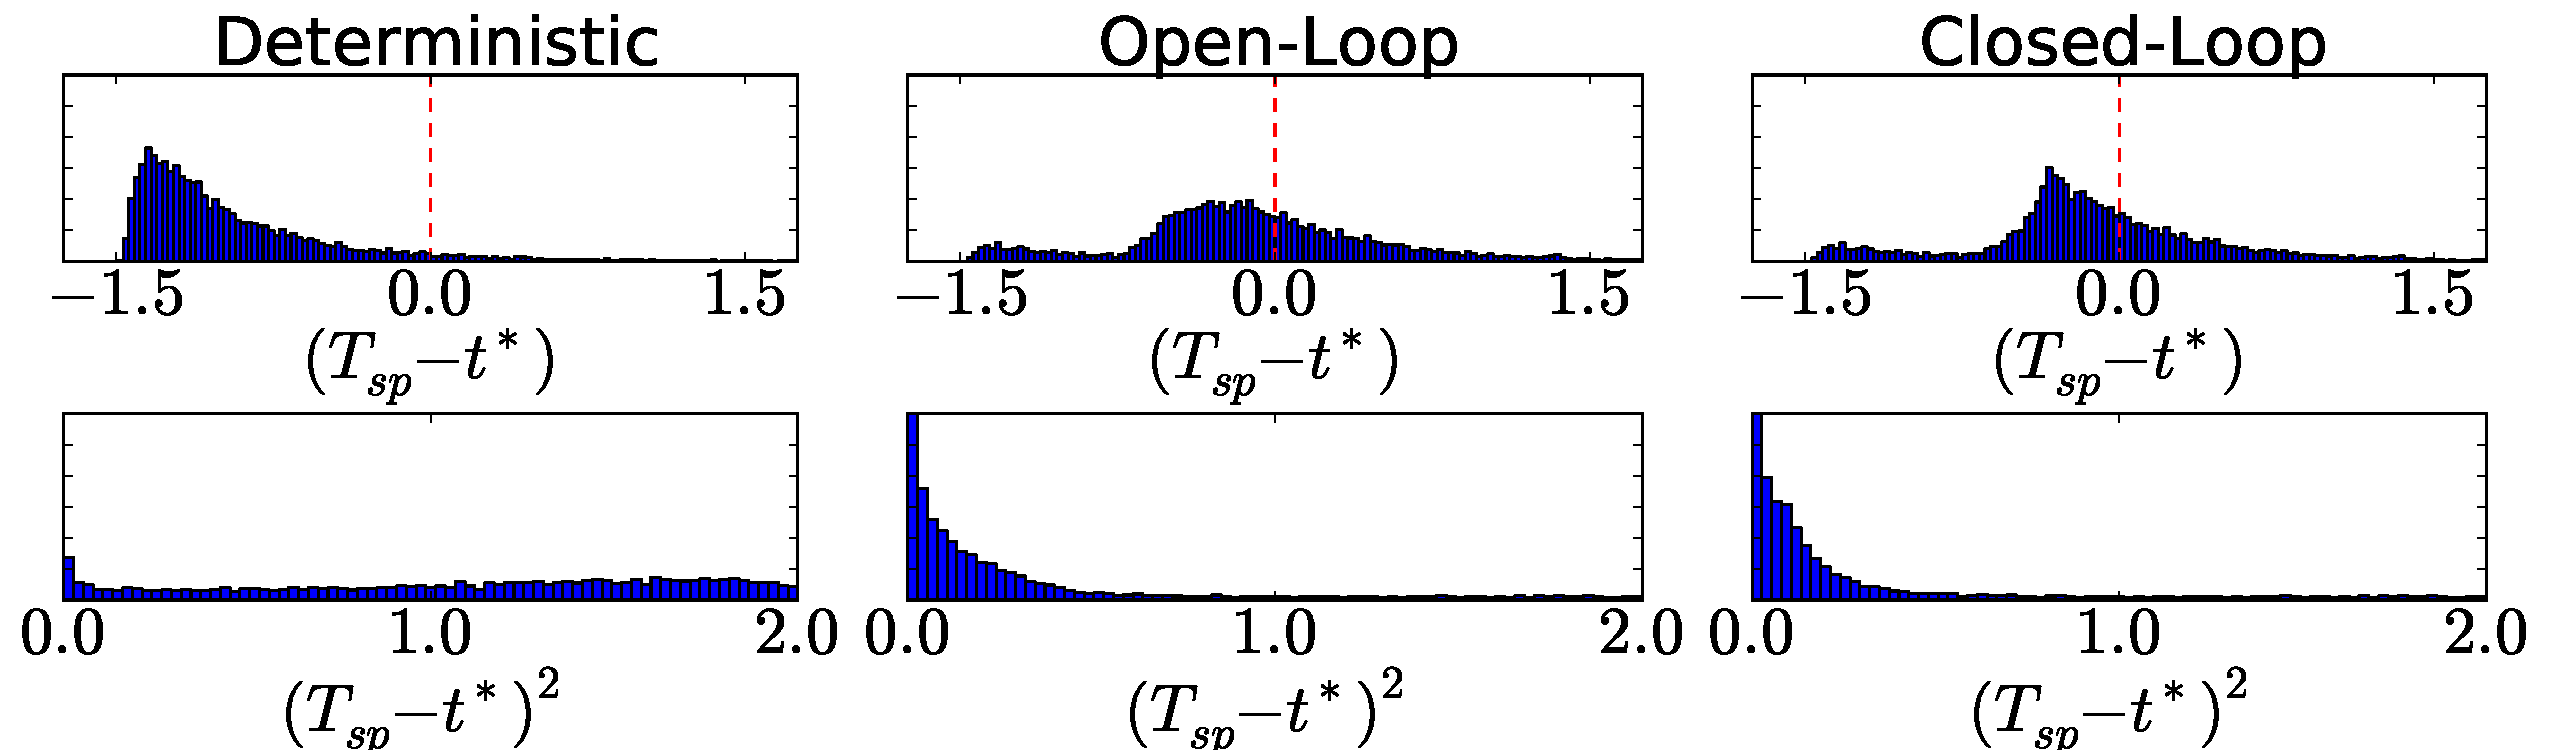
\includegraphics[width=\textwidth]
  {Figs/ControlSimulator/Regimes_subt_HN_errors_hist.pdf}
}\\
  \caption[labelInTOC]{Histogram of the spike timing error for the
  deterministic (left) vs. open-loop stochastic (centre) vs. closed-loop
  stochastic (right) control laws.
  Recall that $\ts$ is the random realized spike time and $\T$ is the target
  spike time.  
  This is for the same problem as in
  \cref{fig:control_trajectories_examples}.
  We have used $N=10000$ sample paths
  to form the statistics.}
  \label{fig:error_histograms_det_vs_openloop_vs_stoch}
\end{center}
\end{figure}
\begin{figure}[h]
\begin{center}
\includegraphics[width=0.99\textwidth]
{Figs/ControlSimulator/Composite_Traj.pdf} 
\caption[]{Three examples for the controlled trajectories using the
deterministic, open-loop stochastic and closed-loop stochastic control approaches.
The plots on the left, A,C,E, are obtained using a value of $\eps=0.001$,
while the plots on the right, B,D,F, use $\eps=0.1$ (for a discussion on the
effect of $\eps$ see \cref{sec:effect_of_eps}). The black vertical line in the plots indicates the
desired spike-time, $\T$. The parameter values are $\m, \tc, \b = [0.2, 0.5,  1.5]$ (Sub-Threshold
High-Noise regime), with $\T = 1.5$. 
The upper plots show the voltage evolution, $X(t)$, while the lower
plots show the applied control, $\a(t)$. Note that the optimal control, $\a(t)$, obtained from
the deterministic and from the open-loop controls are the same across all three
samples.}
\label{fig:control_trajectories_examples}   
\end{center}  
\end{figure}

% \begin{figure}[h]
% \begin{center}
% \subfloat[]
% {
% \label{fig:controlled_traj_ex1}
% \includegraphics[width=0.33\textwidth]
% {Figs/ControlSimulator/SubTHighNoise_Traj0.pdf}
% }
% \subfloat[ ]
% {
% \label{fig:controlled_traj_ex2}
% \includegraphics[width=0.33\textwidth]
% {Figs/ControlSimulator/SubTHighNoise_Traj4.pdf}
% }
% \subfloat[ ]
% {
% \label{fig:controlled_traj_ex3}
% \includegraphics[width=0.33\textwidth]
% {Figs/ControlSimulator/SubTHighNoise_Traj7.pdf}
% }
% \caption[]{Examples for the controlled trajectories using the
% deterministic, open-loop stochastic and closed-loop stochastic control
% approaches. The black vertical line in the plots indicates the desired spike-time, $\T$.
% For the parameter values are $\m, \tc, \b = [.2, .5,  1.5]$ (Sub-Threshold
% High-Noise regime). $\T = 1.5, \eps = 0.001$. The three panels from left to
% right are three different realizations of the model dynamics. On the upper
% plots, we show the voltage evolution, $X_t$, on the lower plots we show the
% applied control, $\a(t)$. Note that $\a(t)$ obtained from the
% deterministic and open-loop controls are the same for all three samples.}
% \label{fig:control_trajectories_examples}
% \end{center}
% \end{figure}

\clearpage

\subsection{Multi-Spike Control}
We now turn to the ultimate goal of our analysis, the control of {\sl spike
trains}. In particular, we will generate $M=50$ realizations of $N=16$ spikes
each in an attempt to meet a prescribed spike train. We will focus on two
regimes, the Supra-Threshold regime with either low or high noise. The results
for parameters from the low-noise regime are shown in
\cref{fig:targettrain_cl_lownoise,fig:targettrain_ol_lownoise}, while, the
results for the high-noise regime are shown in
\cref{fig:targettrain_cl_highnoise,fig:targettrain_ol_highnoise}. In all cases,
the target train is obtained by a simulation of the Supra-Threshold High Noise
regime with no additional control, i.e.\ $\a(\cdot) = 0$.

It is immediately clear that while the evoked trains closely follow the target
train in the low-noise case,
\cref{fig:targettrain_cl_lownoise,fig:targettrain_ol_lownoise}, this is a lot
more difficult in the high-noise case,
\cref{fig:targettrain_cl_highnoise,fig:targettrain_ol_highnoise}.

In each figure,
\cref{fig:targettrain_cl_lownoise,fig:targettrain_ol_lownoise,fig:targettrain_cl_highnoise,fig:targettrain_ol_highnoise}
on the top panel we show a smoothed version of the target train vs.\ an
empirical firing rate from the simulations. The red curve is a smoothed Gaussian
kernel applied at the target times where the standard deviation of the kernel is
$\sigma = 0.1$. The blue curve is the empirical firing rate equal to the number
of spikes in a small window divided by the number of realizations and divided by
the width of the window $w_b$. We have used $w_b = 0.1$. In the bottom panels of
\cref{fig:targettrain_cl_lownoise,fig:targettrain_ol_lownoise,fig:targettrain_cl_highnoise,fig:targettrain_ol_highnoise},
we show in detail $10$ out of the $M=50$ realizations.

In the high-noise case, the restricted control is obviously not able to produce
reliable results. A stronger control is needed to obtain the same level of
accuracy in the target. In \cref{fig:targettrain_cl_highnoise_aplus}, we relax
the bound constraints on the control $[\amin, \amax]$ from $[-2; 2]$ to $[-4;
4]$. Then a significantly better tracking of the target train is achieved. Thus,
to control a system under higher noise comes at the price of allowing a more
powerful control signal.

The main question in this section is whether the separate optimization
of each interval independently of the others is a suitable approach when
targeting a whole spike train. In particular, we do not account 
for the possibility that two target spikes occur closely together. Then
it might make sense to attempt generating the first
one a little earlier, on average, to give more time to generate the
second. For example, in figs. 6 and 7, the 13th target spike is
successfully produced, but the 14th target spike occurs so soon after
that in all trials it is delayed. However, if the target interspike
intervals are within reasonable reach of the neuron, this is not a problem.

% In \cref{fig:targettrain_cl_highnoise_aplus}, we see that once we relax the
% bound constrains on the control $\amin, \amax$ from $[-2,2]$ to $[-4,4]$, we can
% achieve significantly better tracking of the target train.
% 
% Note that the main question in this section is whether the separate optimization
% of each interval independently of the others 'works' when we are working with a
% whole train. In particular, we do not account for the following possible
% occurence, if two target spikes occur closely together, then it might make sense
% to attempt generating the first one a little earlier, on average, to give more
% time to generate the second. At least visually however, we see that this is not
% necessarily a problem in
% \cref{fig:targettrain_cl_lownoise,fig:targettrain_ol_lownoise,fig:targettrain_cl_highnoise,fig:targettrain_ol_highnoise}.
% 
% TODO: I DON''T REALLY KNOW HOW TO ARGUE THIS - IT'S A POSSIBLE PROBLEM, BUT IT
% IS HARD TO SAY WHETHER IT OCCURS IN PRACTICE, WHEN IT OCCURS, DOES IT OCCUR IN
% OUR SIMULATIONS  OR DOES IT NOT\ldots?
 
 


% %%%%%%%%%%%%%%%%%%%%%%%%%%%%%%%%%%%%%%%%%%%%%%%%%%%%%%%%%%%%%%%%%%%% %%%%%%%%%
% SUPER-THRESHOLD REGIME LOW-NOISe: %%%%%%%%%%%%%%%%%%%%%%%%%%%%%%
% %%%%%%%%%%%%%%%%%%%%%%%%%%%%%%%%%%%%%%
\begin{figure}[htp]
\begin{center}
  \includegraphics[width=\textwidth]{Figs/TrainController/SUPT_ln_cl_trains_sim_50.pdf}
  \caption[ ]{How good the {\sl closed-loop} controller is at hitting a target
  spike train. In the panel above, the blue curve is the empirical firing
  rate of $M$ controlled trains.   strategy, the red curve is a
  smoothed-version of the target train. (See text for details of how they are calculated). In the panel below, the
  dashed, red lines indicate the target times, $\t_n$, while the blue dots are
  the realizations of the controlled trains.  
  The parameters from the Super-Threshold, Low-Noise
  regime are used. The target spike train was generated using the model itself,
  with parameters from the Super-Threshold, High-Noise regime, without an applied
  control, $\a=0$.
  There are $N=16$ target spikes and $M=50$ realizations of the control strategy} 
  \label{fig:targettrain_cl_lownoise}
\end{center}
\end{figure}  
\begin{figure}[htp] 
\begin{center}
  \includegraphics[width=\textwidth]{Figs/TrainController/SUPT_ln_ol_trains_sim_50.pdf}
  \caption[ ]{How good the {\sl open-loop} controller is at hitting a target
  spike train.
  The drawn curves have  the same meaning as in
  \cref{fig:targettrain_cl_lownoise}.
  The parameters from the Super-Threshold, Low-Noise regime are used. 
  The target spike train was generated using the model itself, with parameters
  from the Super-Threshold, High-Noise regime, without an applied control, $\a=0$.
  There are $N=16$ target spikes and $M=50$ realizations of the control strategy}
  \label{fig:targettrain_ol_lownoise}
\end{center} 
\end{figure}
%%%%%%%%%%%%%%%%%%%%%%%%%%%%%%%%%%%%%%%%%%%%%%%%%%%%%%%%%%%%%%%%%%%%%
%%%%%%%%%% SUPER-THRESHOLD REGIME HIGH-NOISe:
%%%%%%%%%%%%%%%%%%%%%%%%%%%%%%% %%%%%%%%%%%%%%%%%%%%%%%%%%%%%%%%%%%%%%
\begin{figure}[htp]
\begin{center}
  \includegraphics[width=\textwidth]{Figs/TrainController/SUPT_HN_cl_trains_sim_50.pdf}
  \caption[ ]{How good the {\sl closed-loop} controller is at hitting a target
  spike train. 
  The drawn curves have  the same meaning as in
  \cref{fig:targettrain_cl_lownoise}.
  The parameters from the Super-Threshold, High-Noise regime
  are used. The target spike train was generated using the model itself, with
  parameters from the Super-Threshold, High-Noise regime, without an applied
  control, $\a=0$.
  There are $N=16$ target spikes and $M=50$ realizations of the control strategy}
  \label{fig:targettrain_cl_highnoise}
\end{center} 
\end{figure}
\begin{figure}[htp]
\begin{center}
  \includegraphics[width=\textwidth]{Figs/TrainController/SUPT_HN_ol_trains_sim_50.pdf}
  \caption[]{How good the {\sl open-loop} controller is at hitting a target
  spike train. 
  The drawn curves have  the same meaning as in
  \cref{fig:targettrain_cl_lownoise}.
  The parameters from the Super-Threshold, High-Noise regime
  are used. The target spike train was generated using the model itself, with
  parameters from the Super-Threshold, High-Noise regime, without an applied
  control, $\a=0$.
  There are $N=16$ target spikes and $M=50$ realizations of the control strategy}
  \label{fig:targettrain_ol_highnoise}    
\end{center}
\end{figure}

\begin{figure}[htp]
\begin{center}
  \includegraphics[width=\textwidth]{Figs/TrainController/SUPT_HN_cl_aplus_trains_sim_50.pdf}
  \caption[ ]{Same as \cref{fig:targettrain_cl_highnoise}, but with the control
  constraints, $[\amin, \amax]$ increased to $[-4,4]$ instead of $[-2,2]$.}
  \label{fig:targettrain_cl_highnoise_aplus}    
\end{center}
\end{figure} 
% \clearpage

\section{Effect of energy penalty}
\label{sec:effect_of_eps}
So far we have assumed a low value for the energy penalty parameter,
$\eps$, in the objective defined in \cref{eq:OC_LS_variance_energy}. Our
approach has been to be most concerned with the accurate spiking and
that penalizing energy is rather intended to regularize the control and avoid
excessive chattering of the control between its extreme values, than as a goal
in minimizing energy in its own right. Now, we take some time to explore the
effect of a higher $\eps$ on the optimal controls. Intuitively, a
higher value of $\eps$ will tend to bring the optimal control, $\a^*$, closer
to zero. We make a comparison for the four regimes for both the
closed-loop control and the open-loop control in
\cref{fig:HJB_4regimes_control_different_eps,fig:FBK_Regimes_cs_different_es}.
Indeed, for both the closed-loop and open-loop optimal controls, increasing
$\eps$ tends to reduce the absolute value of $\a^*(t)$. In particular, for the
closed-loop control it tends to broaden the area of transition for
decreasing $x$ when the control swings from its minimal, i.e.\ inhibitory value,
to its maximal, i.e.\ excitatory value. Similarly for the open-loop control,
instead of banging from its minimal bound at the beginning of the interval to
its maximal bound at the end, the optimal control for $\e = 0.1$ tends to have a
more mild transition from a slightly inhibitory to slightly excitatory
values.
  
Note however that increasing $\eps$ has an important effect on the validity of
the approximation, used to form the terminal conditions for the value function,
$\v$, and the adjoint variable, $p$. We assumed that applying $\amax$ is
optimal for $t>\T$. This is indeed true in the limit $\eps \ra 0$. However, even for a
finite value of $\eps$, this may still be the optimal thing to do. Indeed, in
the original calculations, where $\eps=0.001$, see the panels on the left in
\cref{fig:HJB_4regimes_control_different_eps,fig:FBK_Regimes_cs_different_es},
the so-obtained value function {\sl implied} that $\a(x,\T) = \amax$. In
other words, our guess that $\a(x, t) = \amax$ for $t > \T$, is
self-consistent with the so-obtained value function. This is akin to confirming an ansatz. For a higher
value of $\eps$, like $\eps = 0.1$, this is no longer the case. The red curves
on the right-side of \cref{fig:HJB_4regimes_control_different_eps} are no longer
pushed up at $\a = \amax$, and as such it is no longer valid, strictly speaking,
to assume that the value function can be obtained by assuming $\a(t)|_{t>\T} =
\amax$ and then calculating the expected remaining time-to-spike. The exact same
conclusion can be drawn from the open-loop control. There the optimal control
always (almost) reaches its maximum, $\amax$ while choosing $\eps = 0.001$,
this is no longer so for the higher $\eps = 0.1$. In fact, as we mentioned
after \cref{eq:valuefun_TCs}, the correct thing to do for higher values of $\eps$ is
to push the calculation interval to some $t^+ > \T$, apply the same terminal
condition at $t^+$ instead of $\T$ and then solve backwards (either for the
closed- or open-loop control). One will be guaranteed to find some $t^+ > \T$
that works since eventually the quadratic term $(t-\T)^2$ will dominate the
energy term in the objective, which is linear in $t$. We do not explore this
further here.
% CLOSED_LOOP EPS: 
\begin{figure}[htp]
\begin{center}
  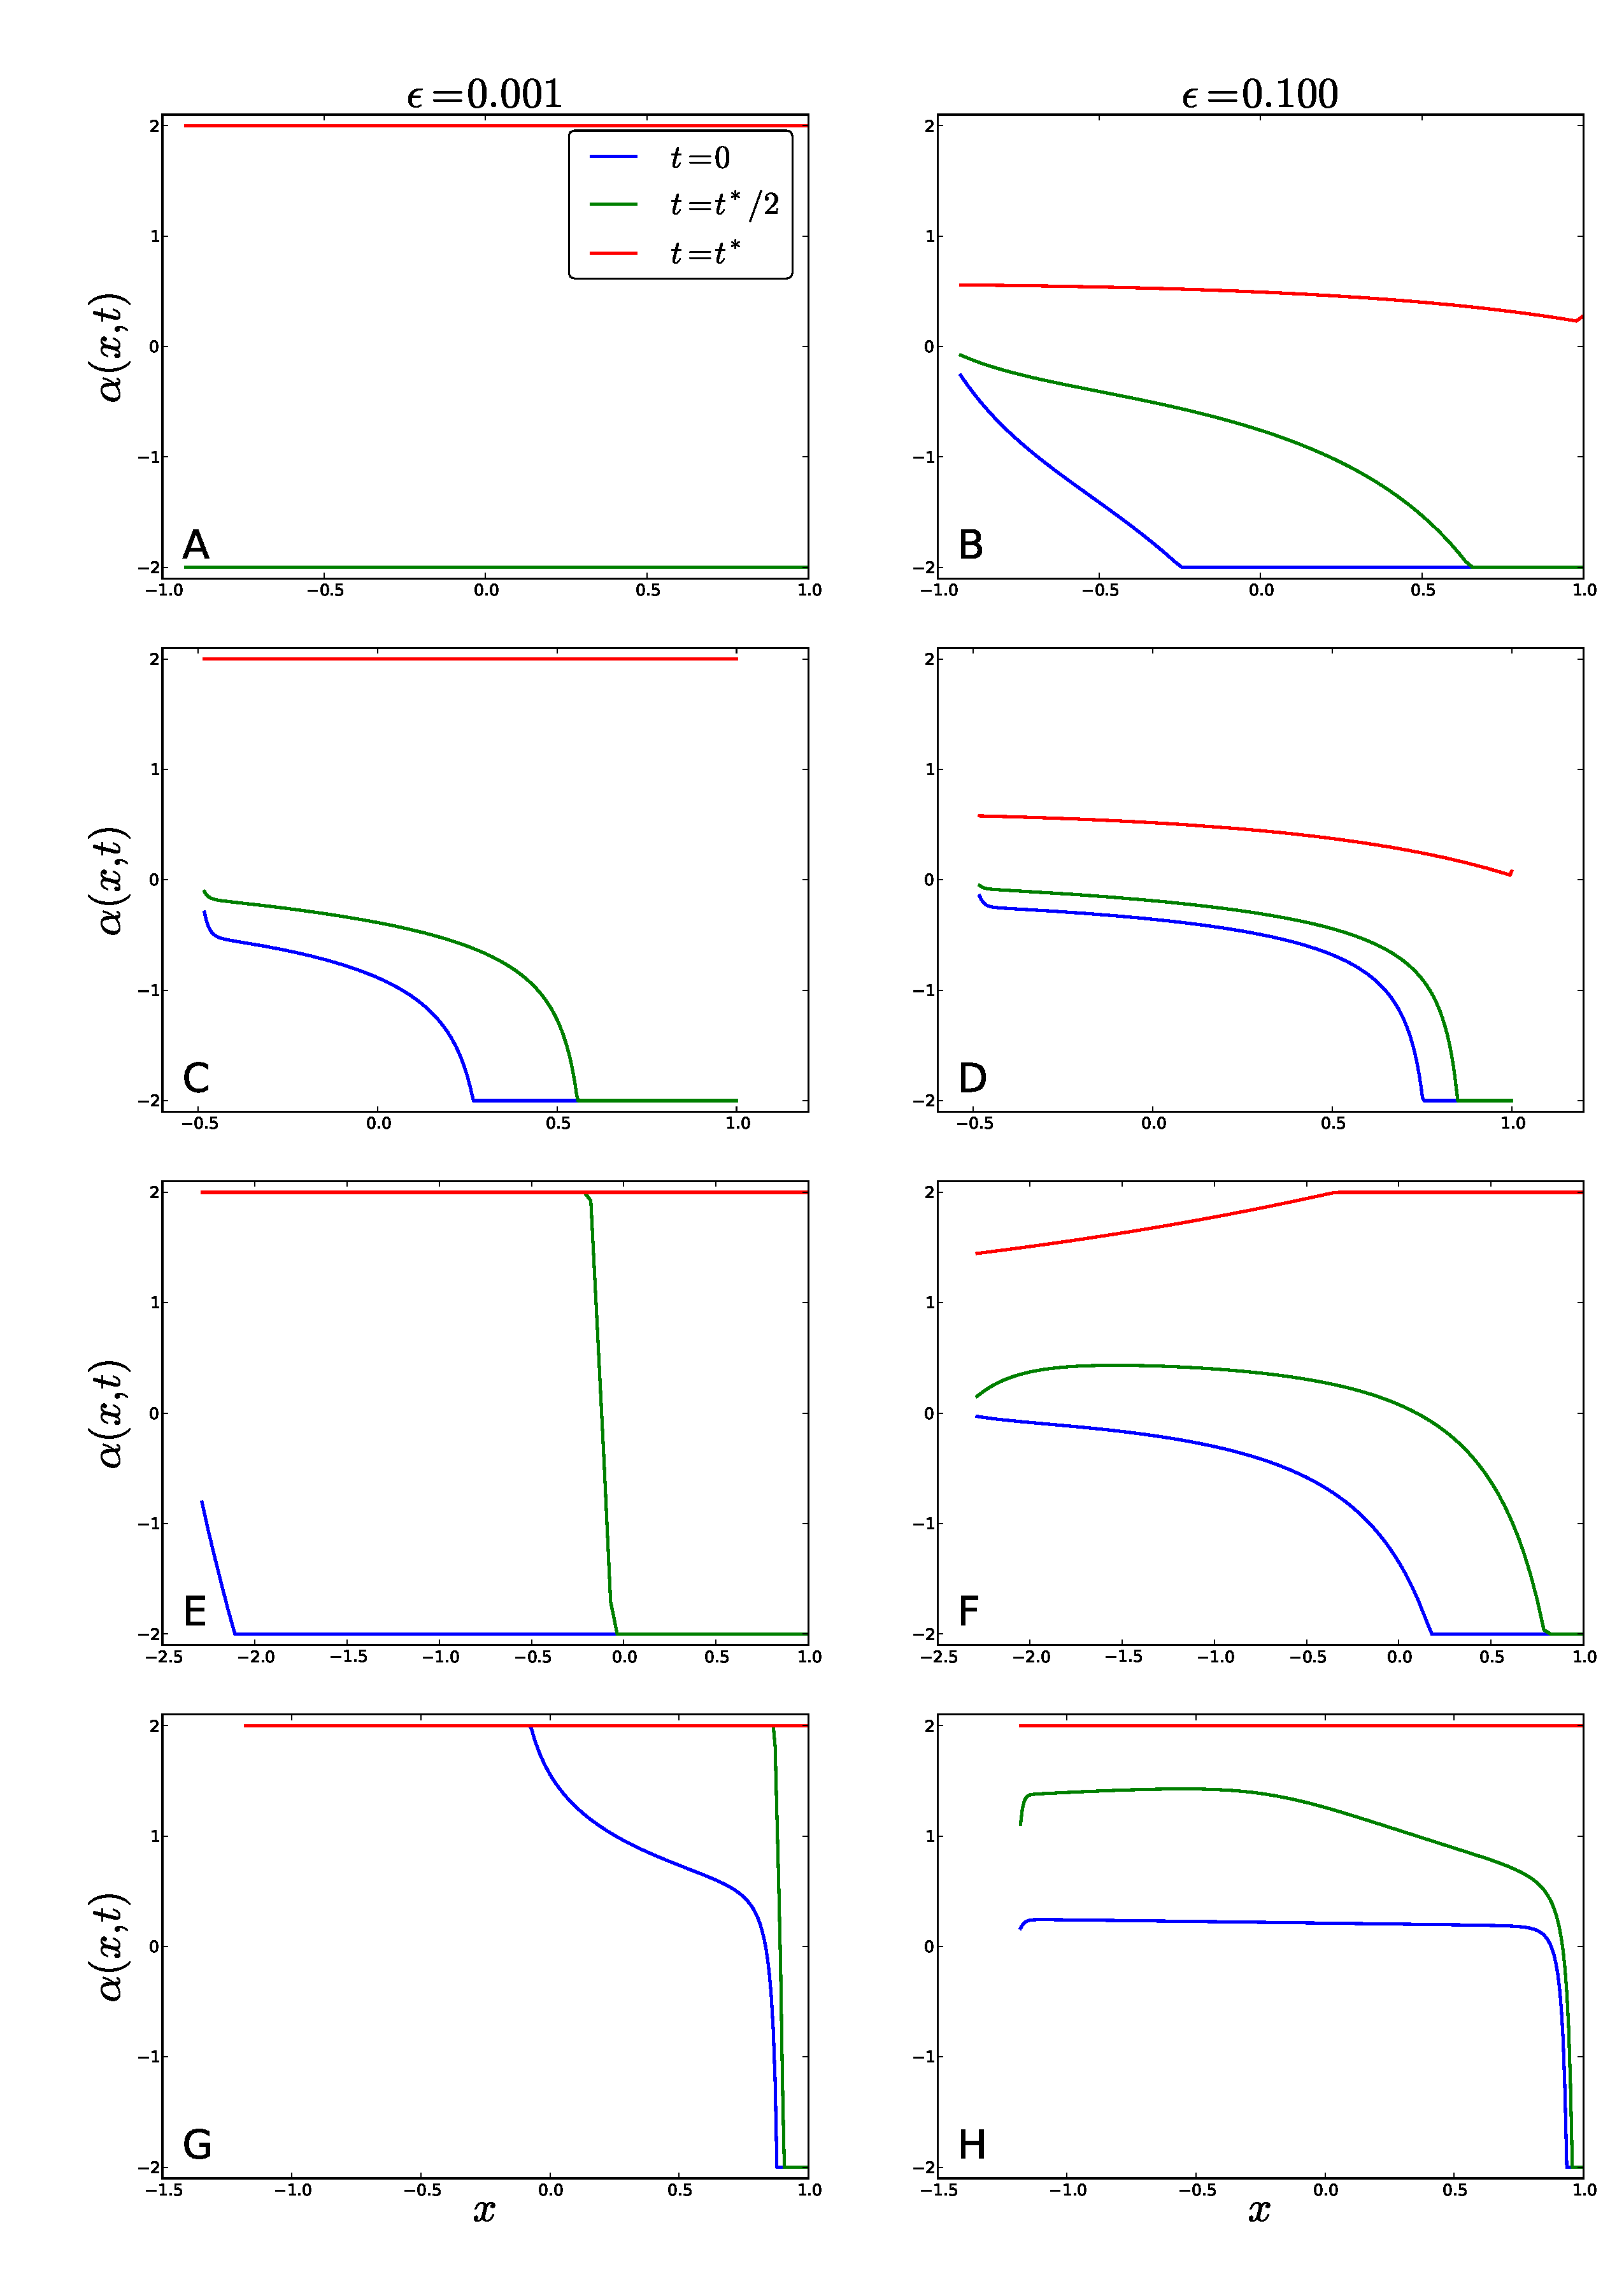
\includegraphics[width=\textwidth]{Figs/HJB/Regimes_eps_comparison.pdf}
  \caption[labelInTOC]{Effect of $\e$ on the closed-loop control. Snapshots of
  $\a(x,t)$ for $t$ fixed, at the start (blue), mid-point (green) and end-point
  (red), for each of the four regimes and different values of $\eps$.
  On the left, we use $\eps = 0.001$ and on the right $\eps = 0.1$.
  The desired spike time is set to
  $\T=1.5$ and the bounds are $\a \in [-2,2]$. 
  A,B)
   Supra-Threshold-Low-Noise 
  C,D) 
   Supra-Threshold-High-Noise 
  E,F)
   Sub-Threshold-Low-Noise 
  G,H)
   Sub-Threshold-High-Noise}
\label{fig:HJB_4regimes_control_different_eps} 
\end{center}
\end{figure}
% OPEN_LOOP EPS:
\begin{figure}[htp]
\begin{center}
  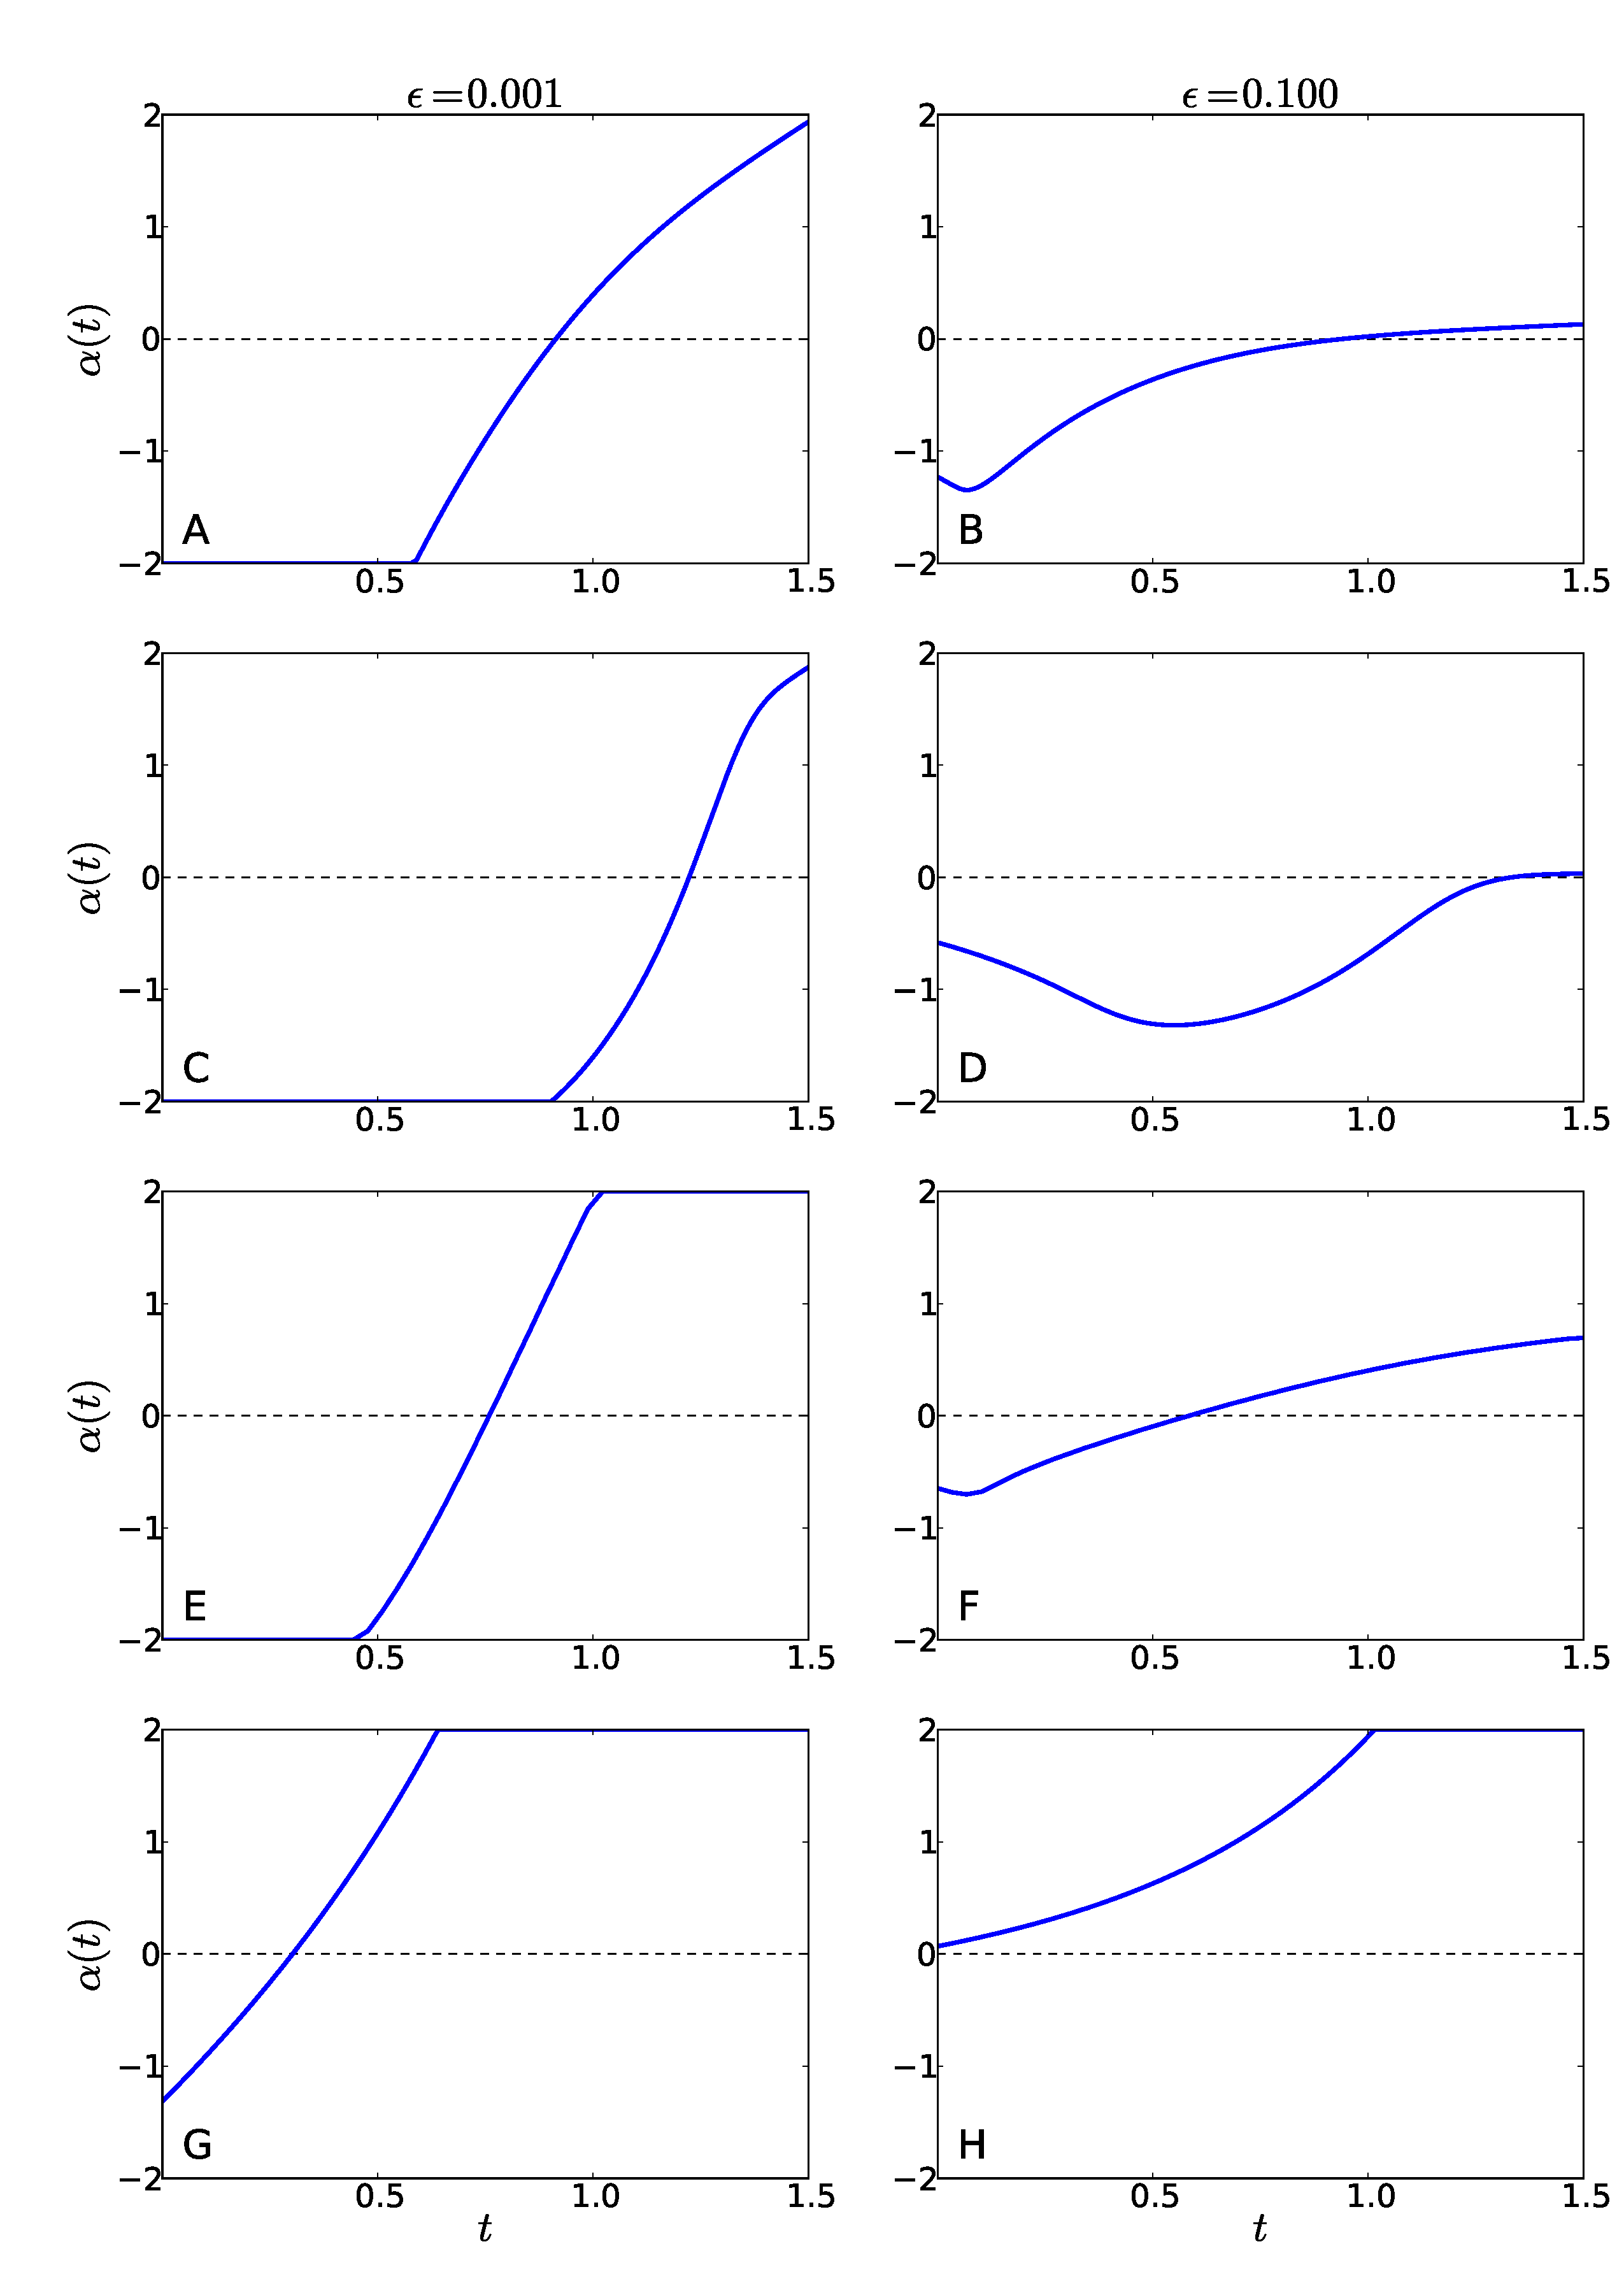
\includegraphics[width=\textwidth]{Figs/FP_Adjoint/Regimes_eps_comparison.pdf}
  \caption[labelInTOC]{Effect of $\e$ on the open-loop control.
  The deterministic time-trajectory of $\a(t)$ for each
  parameter regime as function of time, $t \in [0, \T]$.
  On the left, we use $\eps = 0.001$ and on the right $\eps =0.1$.
  The desired spike time is set to $\T=1.5$ and the bounds are $\a \in [-2,2]$.
    A,B)
   Supra-Threshold-Low-Noise
  C,D) 
   Supra-Threshold-High-Noise
  E,F)
   Sub-Threshold-Low-Noise
  G,H)
   Sub-Threshold-High-Noise}
  \label{fig:FBK_Regimes_cs_different_es} 
\end{center}
\end{figure}

% 
% \begin{figure}[h]
% \begin{center}
% \subfloat[]
% {
% \label{fig:controlled_traj_ex1}
% \includegraphics[width=0.33\textwidth]
% {Figs/ControlSimulator/HighEps_Traj5.pdf}
% }
% \subfloat[ ]
% {
% \label{fig:controlled_traj_ex2}
% \includegraphics[width=0.33\textwidth]
% {Figs/ControlSimulator/HighEps_Traj6.pdf}
% }
% \subfloat[ ]
% {
% \label{fig:controlled_traj_ex3}
% \includegraphics[width=0.33\textwidth]
% {Figs/ControlSimulator/HighEps_Traj0.pdf}
% }
% \caption[]{The effect of higher energy penalty, $\eps = 0.1$.
% Examples for the controlled trajectories using the deterministic,
% open-loop stochastic and closed-loop stochastic control approaches. The black vertical line in the plots indicates the desired
% spike-time, $\T$.
% The parameter values are $\m, \tc, \b = [0.2, 0.5,  1.5]$ (Sub-Threshold
% High-Noise regime). $\T = 1.5, \eps = 0.1$. The three panels from left to
% right are three different realizations of the model dynamics. On the upper
% plots, we show the voltage evolution, $X_t$, on the lower plots we show the
% applied control, $\a(t)$. Note that the optimal control, $\a(t)$, obtained from
% the deterministic and from the open-loop controls are the same across all three
% samples.}
% \label{fig:control_trajectories_examples_high_epsilon}
% \end{center}
% \end{figure}

\section{Robustness of Control}
We have so far assumed that we know the parameters, $\m, \tc, \b$, determining
the dynamics in \cref{eq:X_evolution_uo,eq:current_mu_alpha} exactly. That is,
we assume that the values for $\tc, \b$ used to obtain the controls are the same
as the ones that drive the controlled dynamics. That is slightly naive, as in
any realistic application these will have to be estimated and the estimates will
have some error associated with them. Note that misestimating $\mu$ has the most
immediate and clear effect on the control policy as that amounts to a direct
shift of the control and so for now, let us assume that $\mu$ is estimated
correctly.

Let us then discuss one of the regimes, the Sub-Threshold,
High-Noise regime, and see what is the impact of misspecifying the parameters.

Assume that $\b$ and $\tc$ are underestimated, so that $\b_{est} = \b / 1.5$
and $\tc_{est} = \tc / 1.5$. We will then have: 
$$\mu, \tc_{est}, \b_{est} = \{0.2, 0.5, 1.5 \},$$ which is the control
calculated already for the Sub-Threshold,
High-Noise regime, while the actual simulated dynamics will be driven by
$$\mu, \tc, \b = \{0.2, 0.75, 2.25 \}.$$

We show the effect in
\cref{tab:realized_avg_errors_det_vs_openloop_vs_stoch_misspecified}. Note that
a misspecification of $\b$ should not have a direct influence on the behaviour
of the 'deterministic' controller since it assumes in any case that $\b=0$.
\begin{table}[h]
\begin{center}
 \input{Figs/ControlSimulator/Misspec_MeanSquaredErrors__subt_HN.txt}
 \caption{The effect of misspecifying the parameters. On the left, the
 system parameters and the parameters used to obtain the control are the
 same, i.e.\ correct, on the right, they are misspecified.}
\label{tab:realized_avg_errors_det_vs_openloop_vs_stoch_misspecified}
\end{center}
\end{table}


\section{Discussion}
We have analyzed and computed the optimal control of spikes in two scenarios -
one where the underlying voltage of the neuron is observable to the controller
(closed-loop control) and one where only the spikes are observable (open-loop
control).

Naturally, the ability to control the system is most clearly affected by the
level of the noise. In a sense, the noise acts like an adversary - in our
context it has no beneficial role, except to obstruct precise spiking.
When the level of the noise is high, a stronger control is needed, and
the trade-off between accuracy (hitting the target spikes), possible
damage of the system (the limits of the control) and energy expenditure
has to be considered.

The bias current has a more helpful role at least in our examples, where a
high value of the bias tends to help precise spiking. Of course, where it helps
or hinders depends on the value of the desired spike time - a combination of a
high positive bias and a 'distant' spike time, will tend to be difficult to
control as the system will naturally tend to spike earlier than desired.
In summary, we have found that systems in the Super-Threshold, Low-Noise regime
tend to be most accurately controlled, while the Super-Threshold, High-Noise
regime are the least accurate. 

It should be again noted that we do not require that the controlled cell is
already in the Supra-Threshold regime - the control scheme applies in the same
manner in the Sub-Threshold regime as well.

In both contexts, open-loop and closed-loop, finding the optimal control is
computationally intensive as we numerically solve partial differential
equations. If these algorithms were to be practical in an online setting, some
more work would have to be done in order to ensure they can be computed very
quickly (in the millisecond range) or that they can be pre-computed.

Our work has stayed close to the paradigm of \cite{Ahmadian2011} in
trying to make the neuron spike at a particular time. 
Similiar to them, we have also incorporated into our objective
the minimization of total energy used to achieve our goal, which as discussed in
\cite{Ahmadian2011} is sensible given the potential damage to the cell of
accumulating charge. Furthermore, we have assumed that our control is
constrained in magnitude, which is natural given physical limitations on
equipment and safety considerations. Another possible constraint on the control
is that it is charge-balanced, meaning that its time integral is zero, $\int u
\intd{t} = 0$. Such constraints are most easily posed in the context of
deterministic spiking models like the Phase-Response Curve, see e.g. Danzl et
al. \cite{Danzl2010}. It is possible to add them to the open-loop control, since
the control is still deterministic, but it is non-trivial. It is even less
trivial when one uses Dynamic Programing. In
particular, insisting on charge-balance in our schemes will make it much more
difficult to apply the Terminal Conditions used in deriving both the closed- and
open-loop controls.

% Alternative objectives to spike-timing control in the literature have been
% formulated, most notably the idea of desynchronizing a population of neurons,
% \cite{Nabi2011}, where it is not so important when the neurons spike as long as
% they do not spike at the same time. It is  Maybe you would like to
% write that as a future application, in which case there would be many neurons in parallel to be
% controlled. Alternately, one can imagine that each neuron is firing in the
% suprathreshold regime with a bit of noise, and you wish to apply independent
% controls that makes each one fire the most Poisson-like. If this were achieved
% for each neuron in a population, it would surely have the result of
% desynchronizing them.

As points of outlook, we mention that our scheme can potentially be applied to
produce a periodic train in the face of noise with applications to various
biological pacemakers, or it can also be used to produce the opposite effect - a
random behaviour at the single cell level, for example by specifying a target
train with Poisson-like characteristics.

The novelty in our work is primarily in obtaining a stochastic control scheme,
which is not limited by the intensity of the noise in the system. In fact, by
comparison with the naive 'deterministic' controller, we have shown how wrong
the control strategy can be if we assume that the noise is negligible. Given
this scope, the numerical demands on our scheme are non-trivial, but our
experience and experiments show that these demands can be addressed.
It however remains to be seen whether they can be successfully applied in the lab
and beyond.


\appendix
\section{Calculating the Terminal Conditions for the HJB equation}
\label{sec:valuefun_TCs}
Here we explain how to calculate the first two moments of the remaining
time-to-spike, $\Exp \big[\trem^n \,\Big|\, X(\T) = x, \a(t) = \amax
\big]$, $n=1,2$, which is needed for the terminal conditions for $\v(x,\T)$
and $p(x,\T)$ in, respectively, \cref{eq:OC_LS_HJB_full} and
\cref{eq:adjoint_pde_OU}.

Let
\begin{equation}
\begin{array}{lcl}
\Tone(x) &=& \Exp \Big[\trem \,\,\Big|\, X(\T) = x, \a(t) = \amax
\Big],
\\
\Ttwo(x) &=&
\Exp \Big[\trem^2 \,\Big|\, X(\T) = x, \a(t) = \amax \Big],
\end{array}
\end{equation}
where as before, $\ts-\T$ is the remaining time-to-spike in
\cref{eq:X_evolution_uo}, with the voltage being $X(\T) = x$ at the desired
spike-time $t=\T$ and applying the control $\a(t) = \amax$ afterwards.
Naturally, the $\Ti$'s depend on $x$ and are affected by the value of the
various parameters, $\a,\b,\tc$. We only  need $\Ttwo$ for the TCs in
\cref{eq:OC_LS_HJB_full} and \cref{eq:adjoint_pde_OU}, but $\Tone$ is needed as
an auxiliary. 
  
Analytical expressions exist for $\Ti$, e.g.\ see \cite{Inoue1995}.
However in our experience, they are awkward to work with numerically, especially
as they involve infinite alternating sums which can easily overflow in numeric
calculations. Moreover, they are not particularly convenient if you need $\Ti
(x)$ for a wide range of $x$'s as we do here, since they calculate the value
independently for each $x$. Instead we will follow and slightly extend Jacobs\footnote{Jacobs only discusses how to calculate the first moment
$\Tone$, however it is quite clear from his discussion how to proceed
recursively to obtain any higher moment $\Ti$, by using previously calculated
lower moments. This is what we do here. Moreover the relation between mean exit
times and boundary value problems is discussed in most
introductory books on stochastic processes, see \cite{Oksendal2007} for
example.}, \cite{Jacobs}, in deriving and solving a differential equation for
$\Ti(x)$.

Basically we are calculating the mean squared time to exit an interval
$[\xmin, \xth]$. Theoretically, $\xmin = -\infty$, but for our purposes we will set it to
some finite value and impose reflecting boundaries there. This is a very
good approximation for $\xmin \ll 0$, as long as $\a = \amax >0$.

Let $B(y,t|x) = \Prob[X_0 = y| X(t) = x]$ for a fixed $x$. Then $B$ solves the
following (backward Kolmogorov) PDE
\begin{equation}
-\di_t B = (\m + \a - \frac y\tc)\di_yB - \frac {\b^2} 2 \di_y^2 B.
\label{eq:backward_Xdensity}
\end{equation}
Let $\G(t,y)$ be the survival function for $\ts$ given $X(\T) = y$,
$$\G(t,y) = \Prob[\T>t | X(\T) = y] = \Prob[X(s)|_{s \leq t} \in [\xmin,
\xth] \,\big|\, X(\T) = y].$$
Because the dynamics do not depend explicitly on time, we have
$$
\G(t,y) = \int_\xmin^\xth B(y,t|x) \intd{x}
$$
and so $\G$, being a definite integral of $B$ satisfies the same PDE:
\begin{equation}
-\di_t \G = (\m + \a - \frac y\tc) \di_y\G - \frac {\b^2} 2 \di_y^2 \G,
\label{eq:backward_SDF}
\end{equation}
with the BCs, ICs:
\begin{equation}
\begin{cases}
\G(t,\xth) = 0 & \quad (\ts = t \implies \Prob[\ts>t] = 0)
\\
\di_x \G(t,\xmin) = 0  & \quad (\textrm{due to reflecting boundary for X})
\\
\G(\T, y) = 1. & \quad (\ts \textrm{ is definitely} > \t \textrm{ for } X(\T)
\in (\xmin, \xth) )
\end{cases}
\end{equation}

If we solve the PDE for $\G$ over $t \in [0,\infty)$, then we can calculate
$\Ttwo(x)$ as:
\begin{eqnarray}
\Ttwo(x) &=& \int_0^\infty t^2 \cdot (-\di_t\G(t,x)) \intd{t}
\\
		   &=& \int_0^\infty 2t \cdot \G(t,x) \intd{t},
\end{eqnarray}
assuming it exists.

Since $\Ttwo$ is an integral over time, we can reduce the PDE in
\cref{eq:backward_SDF} for the distribution to an ordinary differential equation
(ODE) for the moments by integrating over time. Multiply both sides of
\cref{eq:backward_SDF} by $2t$, and integrate with respect to time:
\begin{equation}
\int_0^\infty 2t (-\di_t \G) \intd{t}
=
\int_0^\infty  2t \left[ (\m + \amax - \frac y\tc) \di_y\G - \frac {\b^2} 2
\di_y^2 \G\right]
\intd{t}.
\end{equation}
The left-hand side turns out to be $2\Tone$, so
\begin{equation}  
2\Tone
=(\m + \amax - \frac y\tc)   \di_y \Ttwo
- \frac {\b^2} 2
\di_y^2 \Ttwo.
\label{eq:BVP_Ttwo}
\end{equation}
Similarly we can derive an equation for $\Tone$, namely:
\begin{equation}
1
=(\m + \amax - \frac y\tc)   \di_y \Tone
- \frac {\b^2} 2
\di_y^2 \Tone.
\label{eq:BVP_Tone}
\end{equation}
In both cases, the boundary condtions will be:
\begin{equation}
\begin{cases}
\Ti(\xth) = 0 & \quad (\textrm{we are already spking})
\end{cases}
\label{eq:BVP_Ti_BCs}
\end{equation}
Equations \ref{eq:BVP_Tone} and \ref{eq:BVP_Ttwo} can be reduced to first order
differential equations and solved analytically, at least up to some definite integral,
but the analytical solution is not particularly useful or necessary for
numerical calculations. Instead, we opt to calculate the solutions to
\ref{eq:BVP_Tone} and \ref{eq:BVP_Ttwo} directly via an ODE solver, starting
from $T_i(\xth) = 0$ and integrating down for $x  \in [\xmin, \xth]$.
That is how we have obtained the terminal conditions for both $\v(x,\T)$ and
$p(x,\T)$ to apply in, respectively, \cref{eq:OC_LS_HJB_full} and
\cref{eq:adjoint_pde_OU}.

\bibliographystyle{plain}
\bibliographystyle{unsrt}
\bibliographystyle{bmc_article}
\section*{Acknowledgements}
   \ifthenelse{\boolean{publ}}{\small}{}
SD is supported by the Danish Council for Independent Research $\mid$ 
Natural Sciences.
\\ 
AL acknowledges support from NSERC Canada.  
\\
AI is supported by a PGS-D scholarship from NSERC Canada.

\section*{References}
\bibliographystyle{iopartnum}  
\bibliography{library,local} 

\end{document}